\chapter{Testing and Evaluation}
\label{chap:testing_evaluation}

\section{Experimental Methodology}
This chapter evaluates five order book implementations against three core
research hypotheses (\ref{hyp:h1}, \ref{hyp:h2}, and~\ref{hyp:h3}). The benchmarking environment is isolated via
thread-pinning to the canonical x86\_64/WSL2 host (Ryzen 7600X) to ensure
reproducible nanosecond-level precision. Given that WSL2 is a virtualised, 
Hyper-V-managed utility VM~\citep{microsoft_wsl2_arch}, there is an inherent 
"virtualisation tax" and network overhead. However, 
this additional latency is consistent across all tests and does not impact the 
validity of our results. 

To isolate systemic and algorithmic latency, the benchmarking suite incorporates 
two distinct modes. \textbf{Direct mode} focuses on isolating algorithmic 
performance by utilizing thread-pinning and removing transport overhead, thereby 
adhering to the isolation standard defined in~\NFR{3}. This configuration 
allows for the capture of performance trends within the order book 
implementations themselves with minimal external interference. Conversely, 
\textbf{Gateway mode} prioritizes realism by incorporating network transport, 
queueing, FIX parsing, and matching engine processing. This provides a holistic 
view of the end-to-end pipeline (from order submission to consumption by the 
matching engine) in accordance with~\NFR{4}.

When collecting data, we capture significant statistics for four core operations: 
\textbf{insert, cancel, lookup, and matching}. For each of these, we calculate 
a set of metrics, including \textbf{mean latency, standard deviation, 
P99 tail latency, and throughput}, adhering to~\NFR{6}. In gateway and MPSC 
modes, we also decompose these latencies into \textbf{network, queue, and engine 
processing} components to isolate performance bottlenecks. An important 
attribute of our data is to make it reproducible; this is achieved by a 
well-documented benchmarking suite that generates a canonical dataset every time 
it is run, adhering to~\NFR{5}. To guarantee scientific rigour, we rerun our 
benchmarks \textbf{five times} ($n=5$) and average the results to balance 
statistical confidence with measurement stability.

Finally, to evaluate these findings, we refer to the original research hypotheses
(\ref{hyp:h1}, \ref{hyp:h2}, and~\ref{hyp:h3}) as our primary analytical framework. 
To maintain structural rigor, each performance claim in the subsequent sections is 
mapped to its corresponding hypothesis and any relevant NFR IDs.

\section*{Refined Research Hypotheses}

\textbf{H1 (Ordering Structure and Locality).} Index-oriented order-book layouts yield materially lower direct-mode latency than tree-based and sorted-vector designs across most scenarios, with cache behavior as a contributing (not sole) mechanism.

\textbf{Acceptance criteria:} array leads direct-mode mean latency in most scenarios; dense-full gap versus vector remains order-of-magnitude; perf evidence is directionally consistent with higher memory-access pressure in slower variants.

\textbf{H2 (Allocation Strategy in Isolation).} Memory-pooling benefits are implementation- and workload-dependent; pooling does not remove ordering-structure bottlenecks.

\textbf{Acceptance criteria:} pool improves over map only in selected scenarios from the canonical dataset; pool does not approach array where traversal dominates; strong allocator-causality requires dedicated allocation instrumentation.

\textbf{H3 (System-Level Masking).} In gateway mode, network and queue components dominate end-to-end latency, reducing the practical impact of engine-internal data-structure differences except in queue-amplification failure cases.

\textbf{Acceptance criteria:} Network (Net) plus Queue (Que) dominates Engine (Eng) in 34 of 35 non-vector rows; vector dense-full is a clear boundary case showing queue-amplification failure under sustained dense insertion.


\section{Functional Validation}

\subsection{Core Logic and Semantic Parity}
To verify that our order books follow semantic parity~(\NFR{1}), we used 
parameterized contract testing~\citep{fowler_contract_testing} (\FR{6}). Rather than 
testing our order books individually, we applied the same tests to each 
implementation in the form of a contract. We achieved this by using Google Test's 
parameterized suites~\citep{googletest_param}, ensuring each order book was 
verified against identical market scenarios (including happy paths, partial 
fills, and edge cases). This is critical as it guarantees that any subsequent 
performance differences observed are due to architectural efficiency rather than 
logical differences, ensuring fairness in our comparisons~(\NFR{2}).

This testing style was inspired by the \textbf{Ports and Adapters architecture} 
~\citep{cockburn_hexagonal}, employing contracts to reinforce the 
\textbf{Liskov Substitution Principle}~\citep{liskov1987}. Beyond validating 
correctness, this approach improves code maintainability and robustness. 
Furthermore, utilizing the LLVM coverage toolchain~\citep{llvm_cov}, the project 
achieved 100\% coverage across branches, lines, regions, and functions in the 
core order book logic (summarized in Table~\ref{tab:code_coverage_results}), 
providing formal evidence that the benchmarking results are derived from fully 
validated and semantically equivalent components.

\begin{table}[htbp]
    \centering
    \small
    \begin{tabular}{lr}
        \toprule
        \textbf{Metric} & \textbf{Coverage Percentage} \\
        \midrule
        Function Coverage & 100.00\% (96/96) \\
        Line Coverage     & 100.00\% (1355/1355) \\
        Region Coverage   & 100.00\% (572/572) \\
        Branch Coverage   & 100.00\% (370/370) \\
        \bottomrule
    \end{tabular}
    \caption{Code Coverage Results for Core Order Book Logic}
    \label{tab:code_coverage_results}
\end{table}


To obtain a holistic view of the system's performance limits, we integrated a 
range of diverse and plausible market scenarios. These act as a rigorous 
functional test for our implementations, providing insight into how each 
order book performs under varying loads. These scenarios include: 
\begin{itemize}
    \item \textbf{Full Aggressive Matches}: To verify the matching logic's ability 
    to correctly exhaust liquidity and remove orders across multiple price levels.
    \item \textbf{Nested Limit Orders}: To test the data structure's efficiency in 
    maintaining price-time priority across complex book depth.
    \item \textbf{Invalid Entry Handling}: To verify that zero-quantity or illegal 
    price orders are safely rejected without corrupting the internal state.
\end{itemize}
We compared all five implementations against a \textbf{golden reference} derived 
from the \texttt{MapOrderBook} implementation. As the most straightforward translation of 
limit order book logic, it serves as the benchmark to ensure that 
the more complex, high-speed implementations maintain identical logical behavior.

To ensure the statistical validity of the most complex test case, the 
\textbf{mixed} scenario, we define three price-proximity tiers relative to the 
market midpoint. These consist of \textbf{near-spread} activity (orders within 
$\pm$6 ticks of the mid-price), \textbf{deep share} ($\pm$10 to $\pm$50 ticks), 
and \textbf{extreme share} (outliers at $\pm$400 to $\pm$600 ticks), where a 
`tick' represents the minimum price increment of the exchange. As shown in 
Figure~\ref{fig:mixed_profile}, this configuration is validated by capturing the 
branch probabilities within the order generator to confirm the workload 
maintains a heterogeneous distribution rather than collapsing into a single 
regime~(\NFR{1}). This level of transparency in the benchmark generation ensures 
that all subsequent performance claims are strictly bounded by known evidence, 
adhering to~\NFR{9}.

\begin{figure}[htbp]
    \centering
    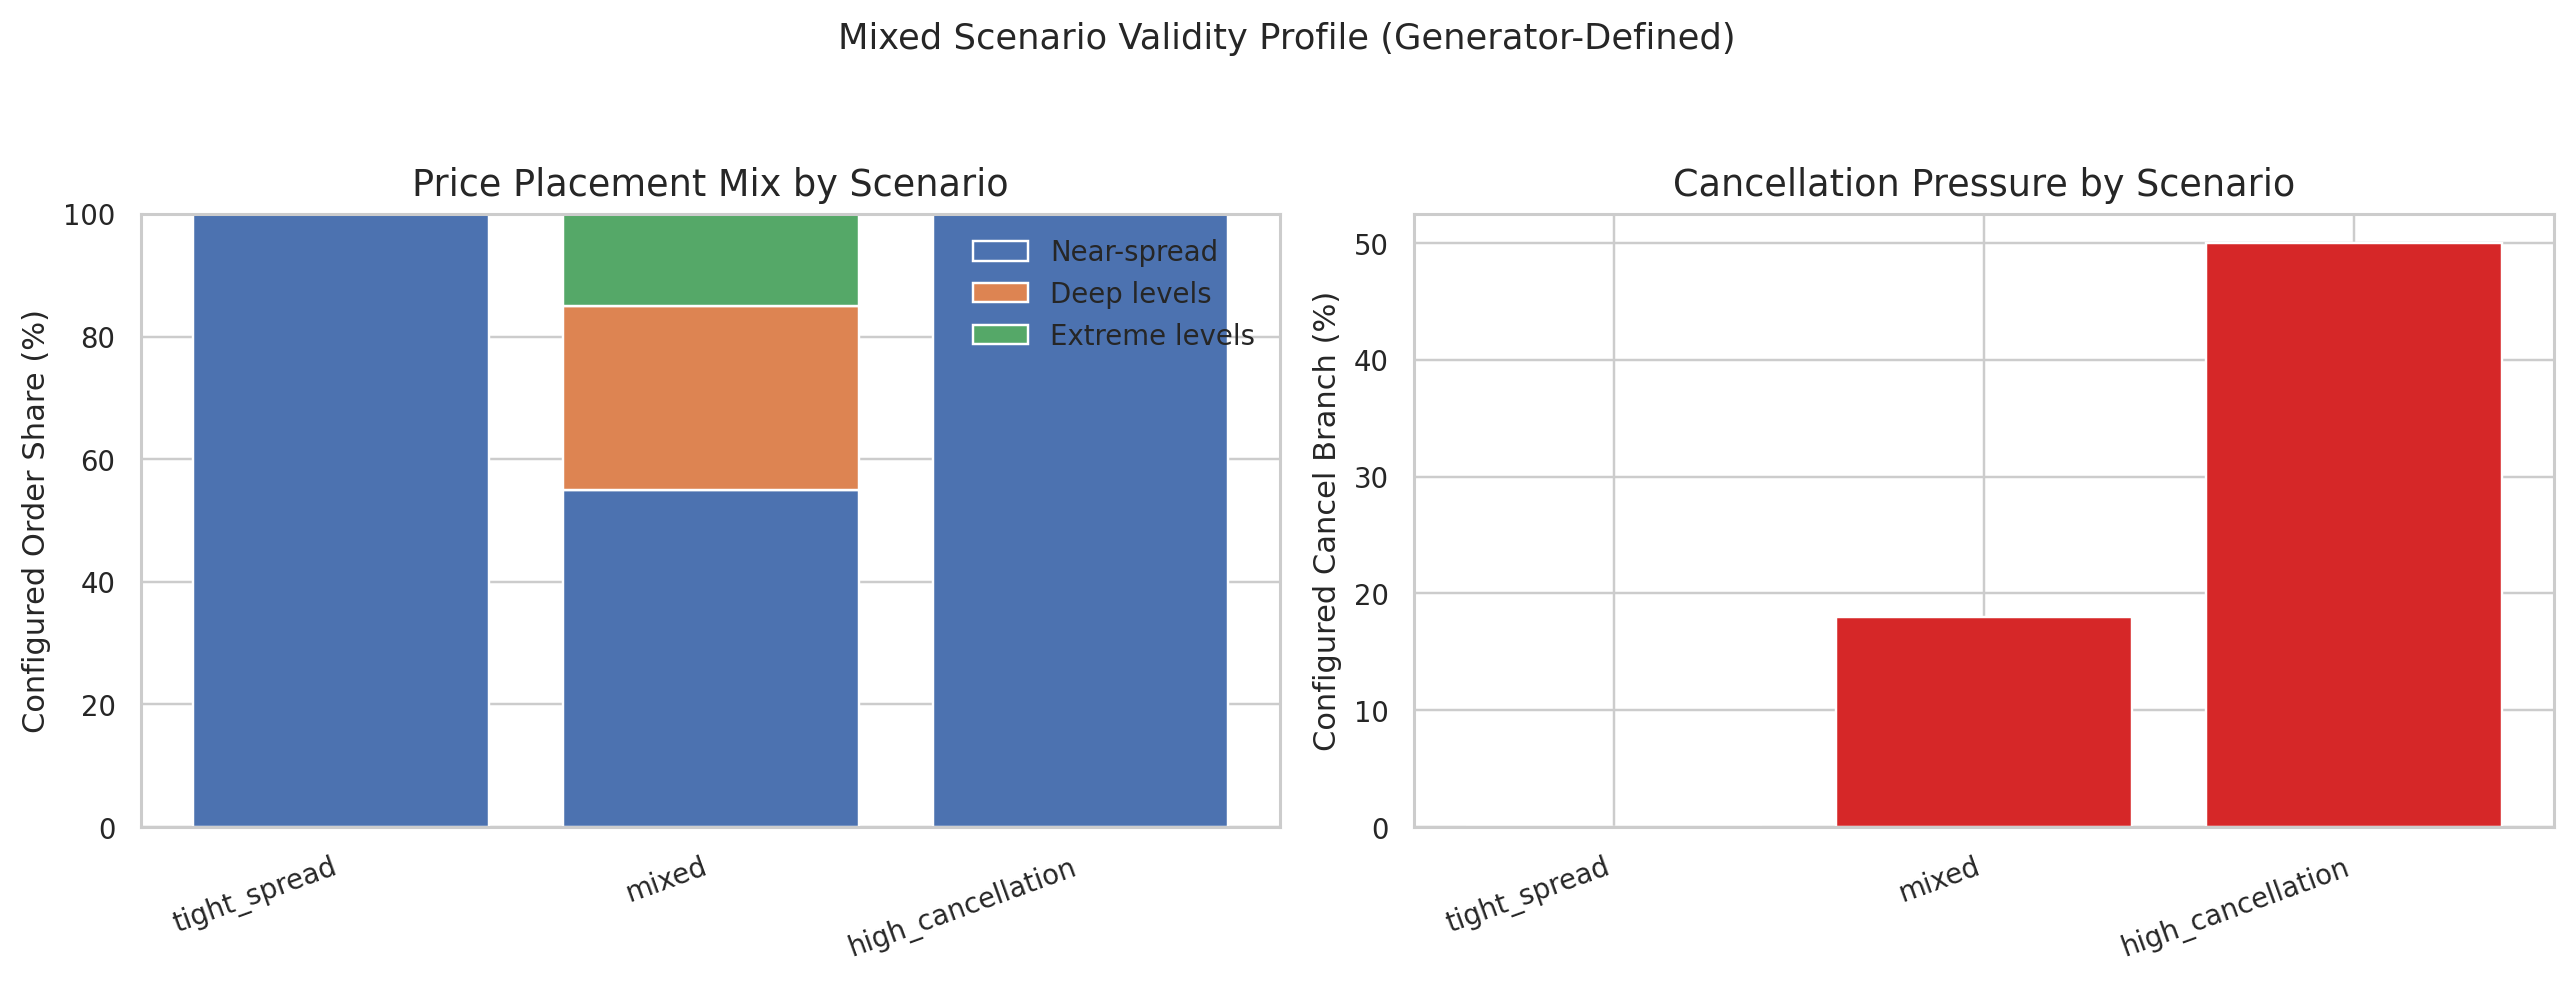
\includegraphics[width=0.8\textwidth]{../plots/scenario_validity/mixed_profile.png}
    \caption{Mixed-scenario profile validation plot. The left panel confirms the 
    55/30/15 distribution across near-spread, deep, and extreme price levels, 
    while the right panel verifies the 18\% cancellation pressure. This validates 
    the generator's output against its theoretical configuration (NFR-1, NFR-9).}
    \label{fig:mixed_profile}
\end{figure}

\subsection{System Pipeline and Integration}
Stepping back from the order book implementations, it was essential to validate the 
entire system pipeline to ensure that functional correctness is maintained from 
the point of entry to the point of execution. This pipeline, illustrated in 
Figure~\ref{fig:system_architecture}, spans from the initial order request 
submitted via \textbf{FIX 4.2}~\citep{fix42_spec} by a gateway client to the 
eventual consumption by the matching engine. 

\begin{figure}[htbp]
    \centering
    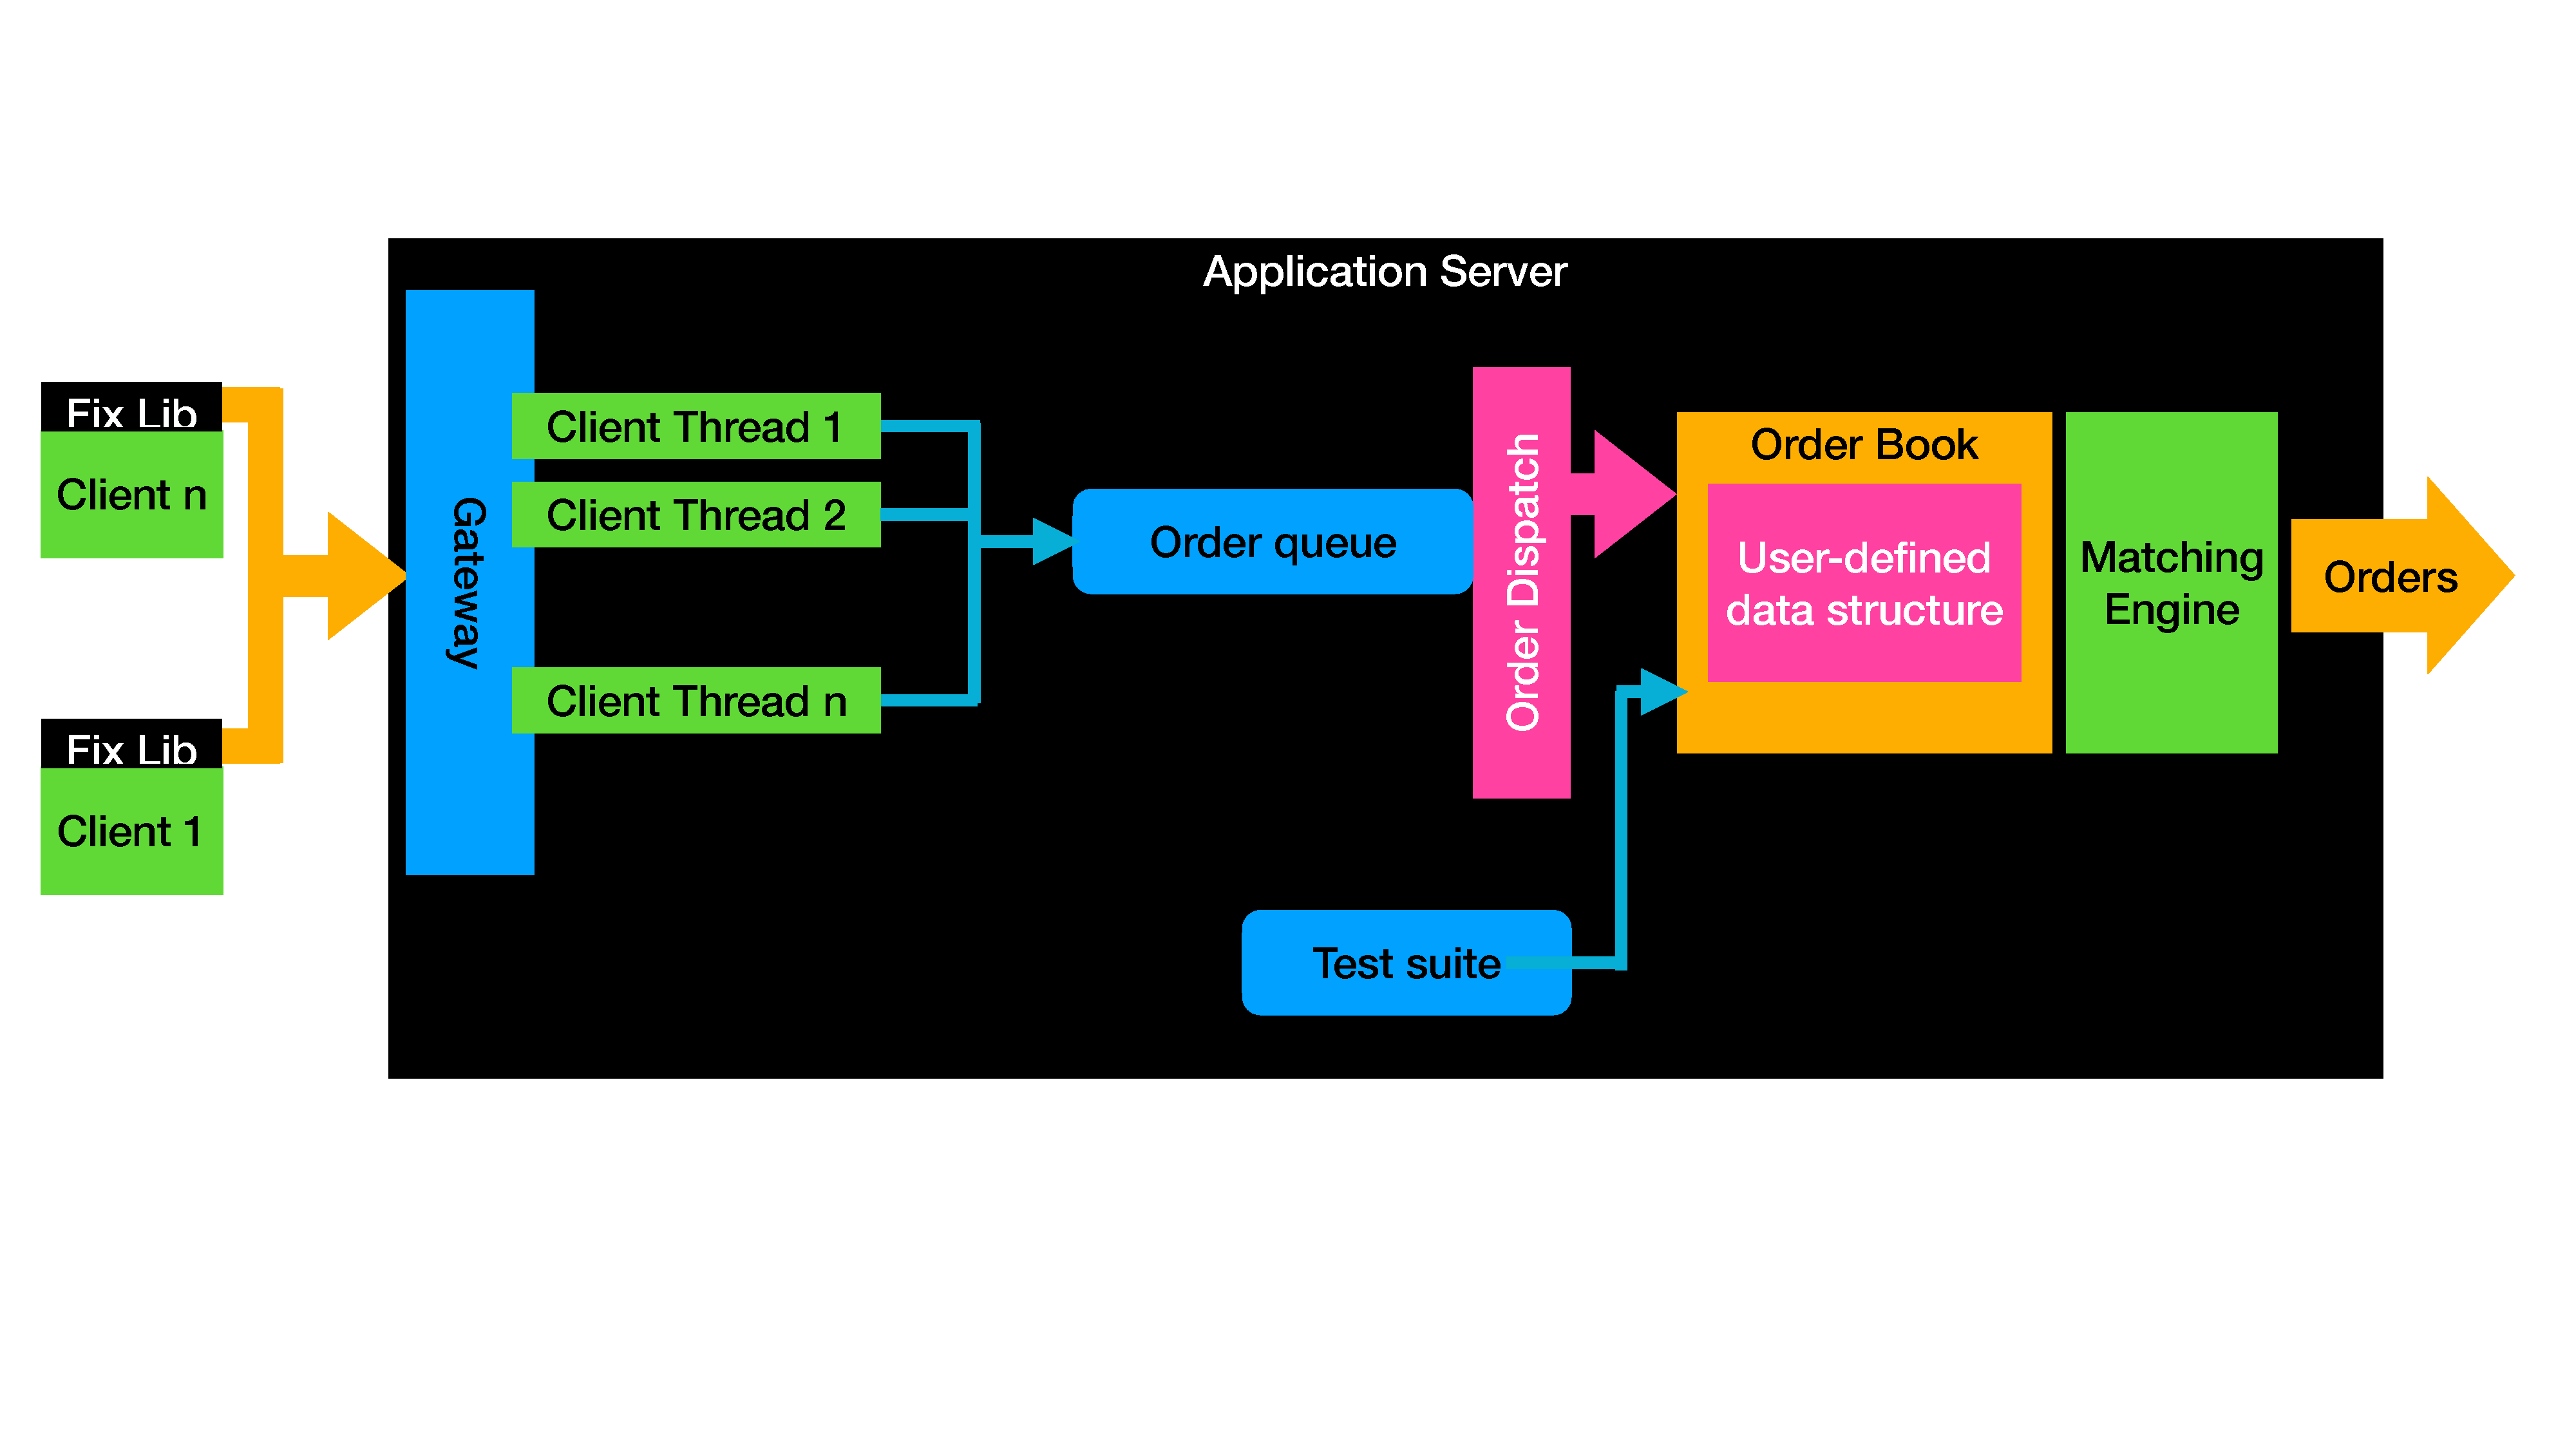
\includegraphics[width=0.9\textwidth]{figures/architecture.pdf}
    \caption{Full System Architecture: From Gateway Client to Matching Engine}
    \label{fig:system_architecture}
\end{figure}

The validation process confirms that incoming \textbf{New Order Single (Tag 35=D)} 
messages are correctly parsed and dispatched into a cache-aligned, 
\textbf{lock-free SPSC InputQueue}. To maintain strict \textbf{traceability}, 
we capture the client's unique order ID (Tag 11) and original transmission 
time (Tag 60~\citep{fix_tag60}) and pair them with an internal \textbf{gateway receipt timestamp}. 
This "triple-timestamp" strategy ensures the integrity of the end-to-end flow; 
by verifying these IDs across the multi-threaded network layer and the 
single-threaded dispatching loop, we confirm that no orders are lost or 
reordered during transport. The validation process confirms that the 
\textbf{New Order Single (Tag 35=D)} message is correctly mapped to internal 
C++ structures as summarized in Table~\ref{tab:fix_mapping}.

\begin{table}[htbp]
    \centering
    \small
    \begin{tabular}{llll}
        \toprule
        \textbf{Tag} & \textbf{FIX Field Name} & \textbf{Example Value} & \textbf{Internal C++ Mapping} \\
        \midrule
        35 & MsgType & D & \texttt{NewOrderSingle} \\
        11 & ClOrdID & 1001 & \texttt{OrderId id} \\
        54 & Side & 1 (Buy) & \texttt{Side::Buy} \\
        38 & OrderQty & 7 & \texttt{Quantity quantity} \\
        44 & Price & 130 & \texttt{Price price} \\
        60 & TransactTime & 123456789 & \texttt{Timestamp sendTimestamp} \\
        \bottomrule
    \end{tabular}
    \caption{Mapping of FIX 4.2 Application Tags to Internal C++ Order Structures}
    \label{tab:fix_mapping}
\end{table}

\subsection{Scaling and Stress Testing}
While the primary architecture uses a custom-built, wait-free \textbf{Single-Producer 
Single-Consumer (SPSC)} queue for learning and simplicity, we also needed to 
test how the system behaves under producer contention. To achieve this, we 
integrated an open-source \textbf{Multi-Producer Multi-Consumer (MPMC)} queue 
from the \textbf{Moodycamel} library~\citep{moodycamel_concurrentqueue}. By 
running this queue in a single-consumer configuration, we were able to evaluate 
how the system behaves under producer contention from multiple concurrent 
clients pushing into the matching engine. Both queue implementations were 
subjected to the same functional validation to ensure that the choice of 
transport did not affect the final order book state.

The \texttt{FIXParser} was also verified to ensure it behaves correctly during 
fragmentation (where the network stream is split into multiple packets) by 
successfully reassembling messages. The queue was tested for back-pressure 
handling; if the 1024-deep queue reaches capacity, a \texttt{push()} call will 
fail, with the expected behavior being that the client is alerted rather than 
the system crashing. Finally, Moodycamel's MPMC queue was integrated to ensure 
that the system maintains stability and does not significantly degrade in 
performance when multiple concurrent clients are querying the engine at the 
same time.

\subsection{Gateway Simulation Boundaries and Validation}
To ensure the end-to-end performance results are technically sound, we 
will define the boundaries of the Gateway simulation. 
As identified in Chapter 4, the benchmark utilises a \textbf{Loopback (AF\_INET)} 
configuration where the \texttt{MockClient} and \texttt{TCPOrderGateway} 
communicate via the local interface (\texttt{127.0.0.1}). 

This setup was validated to confirm that it correctly exercises the full 
\textbf{Linux TCP/IP stack}, including the overhead of system calls 
(\texttt{send}, \texttt{recv}, \texttt{select/poll}), kernel buffer 
copies (\texttt{sk\_buff}), and the associated context switching jitter. 
However, because the client and server reside on the same physical host, 
this environment eliminates the latency of physical network media (cables) 
and NIC hardware processing (e.g., PCIe bus latency). 
Consequently, the absolute results recorded in the "Net" component represent 
a \textbf{theoretical lower-bound} for system latency, effectively isolating 
the "software networking tax" from the "physical hardware tax."



\section{Throughput Results}
\label{sec:throughput_results}
In this section we will work to evaluate hypotheses \ref{hyp:h1} and
\ref{hyp:h3} by analysing
the throughput of the system. The throughput of the system will be analysed
in direct mode and gateway mode, isolating the operations first, and then taking
into account realistic overheads. 

The throughput results in direct mode work to verify~\ref{hyp:h1}, which
claims that order books with index-based layouts will be faster than those with
search trees or sorted vectors. We can see evidence for this claim by observing
the greatest throughput of 8,921,972~ops/s achieved by the \textbf{ArrayOrderBook}.
It significantly beats the other order books: the \textbf{PoolOrderBook} comes
second at 7,002,000~ops/s (27.4\% lower), followed by \textbf{HybridOrderBook}
at 6,789,183~ops/s (31.4\% lower), \textbf{MapOrderBook} at 6,652,726~ops/s
(34.1\% lower), and \textbf{VectorOrderBook} at 6,084,046~ops/s (46.7\% lower).
These figures are derived by averaging throughput across seven benchmark scenarios
(tight spread, fixed levels, dense full, sparse extreme, worst case FIFO, mixed,
and high cancellation), each of which exercises a mix of insert, cancel,
lookup, and match operations, adhering to~\NFR{6}.
Although \textbf{ArrayOrderBook} wins here, it is not without its downsides.
When using index-based order books, the implementer is forced to define a fixed
range of valid prices and a discrete tick size. Additionally, logic must be
provided to handle orders whose prices fall outside the maximum and minimum
values of the order book, or that do not fall exactly on a price level.
In general, traders may not be happy with these restrictions, reducing the
accessibility of the exchange.
The second-place \textbf{PoolOrderBook}, by contrast, imposes no such
price-range constraints. Its competitive throughput can be attributed to
its custom memory pool, which eliminates dynamic heap allocation on
the critical path and reduces allocator overhead compared to the
pointer-chasing traversal of \textbf{MapOrderBook}.


\begin{table}[htbp]
    \centering
    \small
    \begin{tabular}{lrr}
        \toprule
        \textbf{Implementation} & \textbf{Direct Mode (ops/s)} & \textbf{Gateway Mode (ops/s)} \\
        \midrule
        ArrayOrderBook   & 8,921,972 & 1,063,760 \\
        MapOrderBook     & 6,652,726 & 1,057,882 \\
        VectorOrderBook  & 6,084,046 &   985,022 \\
        HybridOrderBook  & 6,789,183 & 1,060,957 \\
        PoolOrderBook    & 7,002,000 & 1,069,759 \\
        \bottomrule
    \end{tabular}
    \caption{Mean Throughput Across All Implementations in Direct and Gateway Mode}
    \label{tab:throughput_results}
\end{table}

The gateway mode results support~\ref{hyp:h3}. In a realistic exchange
with overheads in the form of the network and queues, these additional latencies
mask the performance differences between order books. In direct mode, the throughput
spread across all implementations reached 46.7\% (8,921,972 vs 6,084,046~ops/s).
In gateway mode, that spread compresses to just 7.6\% (1,069,759 vs 985,022~ops/s),
with four of the five implementations clustering within 1.2\% of each other.
The data indicates that this convergence is a direct consequence of the network
component consuming approximately 99.9\% of total end-to-end latency for all
non-pathological implementations (see Table~\ref{tab:gateway_decomposition}),
in accordance with~\NFR{4}. The ordering structure of the engine becomes
largely irrelevant when the transport stack dominates the pipeline to this degree.


\section{Latency Analysis - Direct Mode}

This section provides a deeper analysis of the per-operation latencies across all
order book implementations, strictly in direct mode to isolate data structure
behaviour from transport overhead. The results are examined across a range of
market scenarios to highlight the strengths and weaknesses of each design
under different types of market activity. These observations are then used to
evaluate~\ref{hyp:h1} and~\ref{hyp:h2}.


Table~\ref{tab:direct_mean_latency} shows that the fastest book is the
\textbf{ArrayOrderBook}, achieving a mean insert latency of just 15.2~ns.
This represents a 1.85x improvement over \textbf{MapOrderBook} (28.2~ns),
a 1.98x improvement over \textbf{PoolOrderBook} (19.8~ns), and a striking 
9.6x improvement over \textbf{VectorOrderBook} (145.5~ns).
The reason the array data structure yields better performance over the other
order book structures comes down to mechanical sympathy~\citep{fowler2011lmax}. Because elements
in an array are contiguous, they are more cache-friendly~\citep{patterson2013computer}. During a cache hit,
the processor is able to return contiguous elements in the same cache lines,
whereas tree structures such as \textbf{MapOrderBook} do not exhibit this
behaviour since each node in the tree may reside at an arbitrary heap address.
To provide empirical support for these findings, absolute performance counters were
recorded in direct mode using Linux \texttt{perf stat} for pinned, single-core
benchmarks~\citep{linux_perf}. L1 data-cache and branch prediction metrics were
collected across the \texttt{mixed} and \texttt{dense\_full} scenarios.
In the \texttt{mixed} scenario, \textbf{ArrayOrderBook} recorded 843,745 L1 data-cache
misses and a 1.52\% branch miss rate, compared to 1,392,193 misses and a 1.58\%
branch miss rate for \textbf{MapOrderBook}.
The performance gap is most evident in the \texttt{dense\_full} scenario:
\textbf{VectorOrderBook} recorded a severe 144,837,499 L1 misses and
executed 366,302,717 branch instructions (12x the volume of \textbf{ArrayOrderBook}),
consistent with the overhead of O(n) sorted insertion.
Furthermore, while the \textbf{PoolOrderBook} benefits from cache locality, it
exhibits the highest branch miss rate of 7.36\% in the \texttt{mixed} scenario,
explained by the additional conditional logic required for custom pool management.
These measured results validate that the \textbf{ArrayOrderBook}'s advantage
stems from a combination of superior cache hit-rates and a branch-predictor-friendly
execution path, in accordance with~\NFR{8}.

\subsection{Scenario-Specific Latency Trends}
\label{subsec:scenario_latency}
From analysing order book performance across different market scenarios, we have been
able to understand better when the order books perform best. In \texttt{mixed} and
\texttt{fixed\_levels}, the performance gap between the fastest order books - \textbf{Array},
\textbf{Map}, and \textbf{Hybrid} - is small (within ${\sim}10$~ns of each other). In
these cases, the price levels are shallow (a realistic market scenario), so there is a
smaller collection of order prices within the order book. The advantage that follows is
that the underlying data structure is more likely to fit within a CPU's L1 or L2 cache.
This is why performance differences are small in these cases. To really stress test our
order books, we engineered the \texttt{dense\_full} scenario. We create 2,000 price
levels in the order book under this circumstance, where each level is filled at any
given time. The real strengths and weaknesses of our order books are highlighted under
this load.

\begin{figure}[htbp]
    \centering
    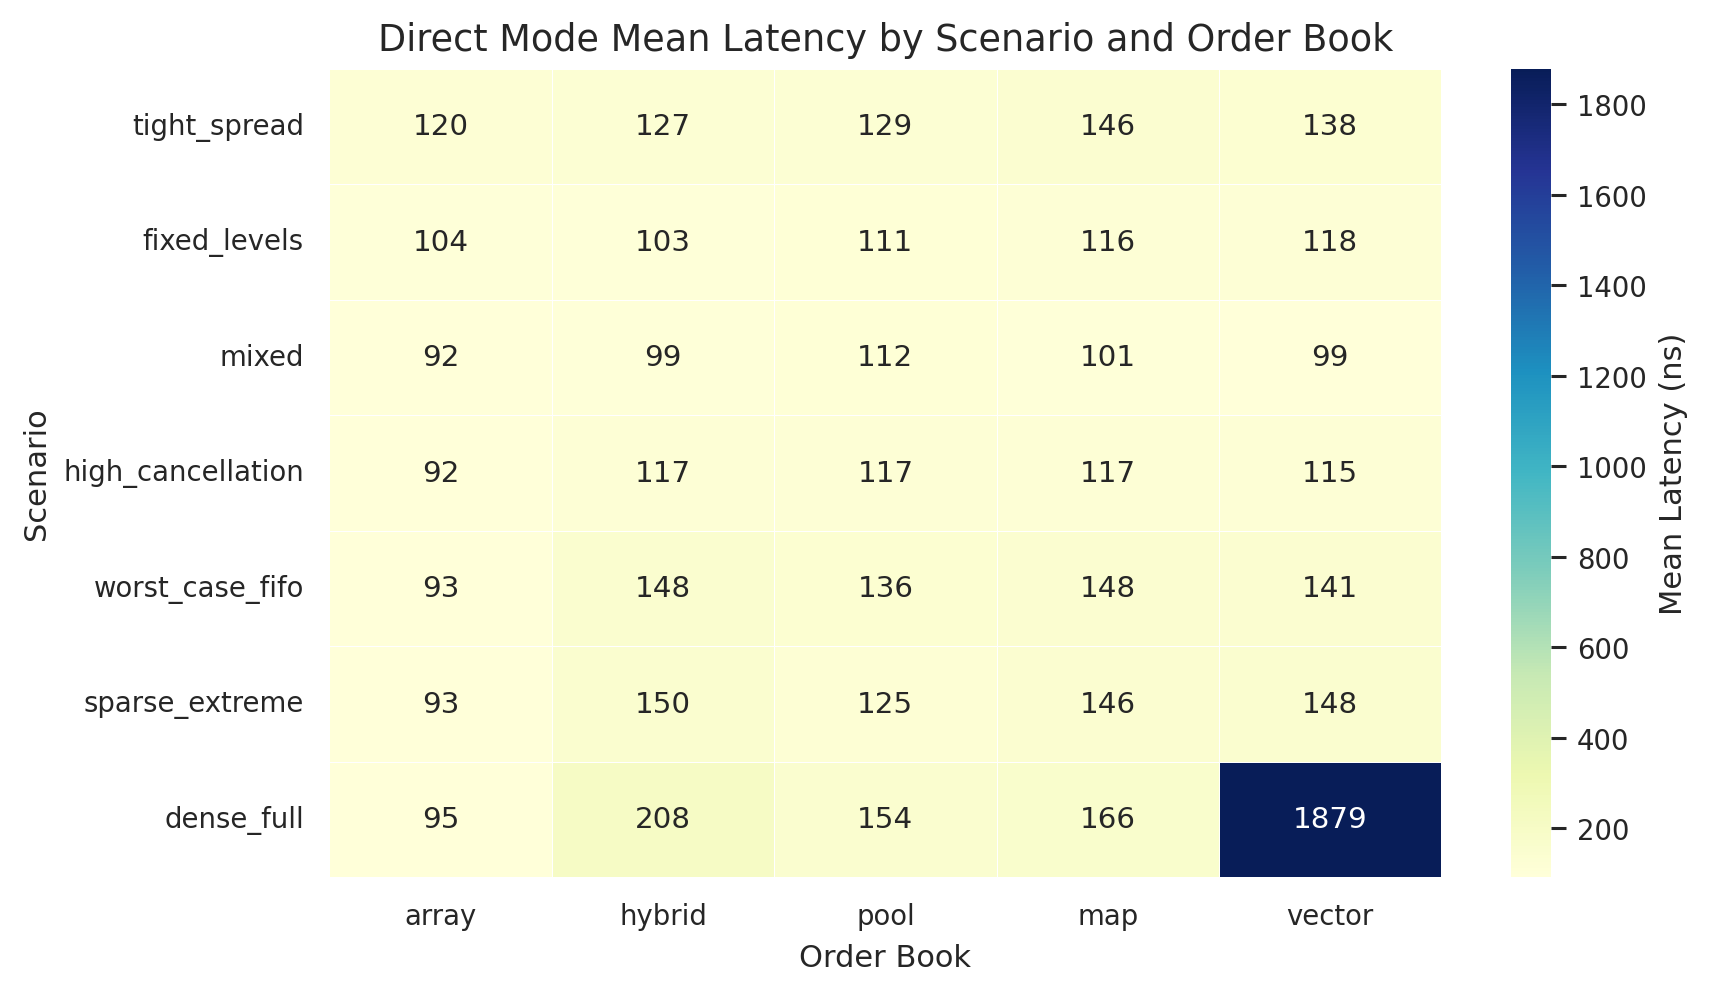
\includegraphics[width=0.8\textwidth]{../plots/direct/latency_mean_heatmap.png}
    \caption{Direct-mode mean latency heatmap across scenarios and order book 
    implementations. Array is the fastest implementation in six of seven 
    scenarios, while hybrid is narrowly fastest in tight\_spread.}
    \label{fig:latency_mean_heatmap}
\end{figure}

The \textbf{VectorOrderBook} exhibits the largest degradation in latency, increasing
from 138.41~ns to 1,878.97~ns in the \texttt{dense\_full} scenario. This is likely due
to the sorted vector having to shift a large number of elements in memory during
frequent insertions. Additionally, this shifting causes a cascade of L1 data-cache
misses - a mechanism reinforced by the Linux \texttt{perf} results,
which recorded 144,837,499 L1 misses and executed 366,302,717 branch instructions for
the vector implementation. To put this in perspective, under the exact same \texttt{dense\_full}
workload, the vector implementation suffered \textbf{216x more L1 cache misses} and
executed \textbf{12x more branch instructions} than the \textbf{ArrayOrderBook}
(which recorded only 670,762 misses and 30,567,574 branches). These results 
strongly indicate that sorted-vector designs
in HFT are unscalable as the order book grows, especially in deep books. A strong trend
among all scenarios is the resilience of the \textbf{ArrayOrderBook}. It stays between
91~ns and 120~ns in all cases, likely due to the $O(1)$ direct index mapping. As a
consequence of this, the algorithmic complexity of operations such as inserting,
cancelling, and looking up orders is identical whether there are 10 or 10,000 price
levels. This provides strong empirical support for~\ref{hyp:h1}.
At the same time, outside \texttt{dense\_full}, the vector implementation is not 
uniformly poor: it beats the map in four of six direct-mode scenarios 
(\texttt{tight\_spread}, \texttt{mixed}, \texttt{high\_cancellation}, and 
\texttt{worst\_case\_fifo}), but these gains are small relative to the 
dense-book regression.

While the \textbf{VectorOrderBook} is included in the mean latency summaries, it 
is excluded from the relative slowdown heatmap in 
Figure~\ref{fig:latency_slowdown_vs_best_heatmap}. This is a deliberate 
aesthetic and analytical choice: since the vector implementation exhibits a 75x 
degradation in \texttt{dense\_full}, its inclusion compresses the colormap scale 
for all other scenarios, masking the subtle performance trade-offs between the 
more competitive implementations. By excluding the vector outlier, the 
high-resolution differences between index-based and tree-based structures become 
visually discernible across all market regimes.

\begin{figure}[htbp]
    \centering
    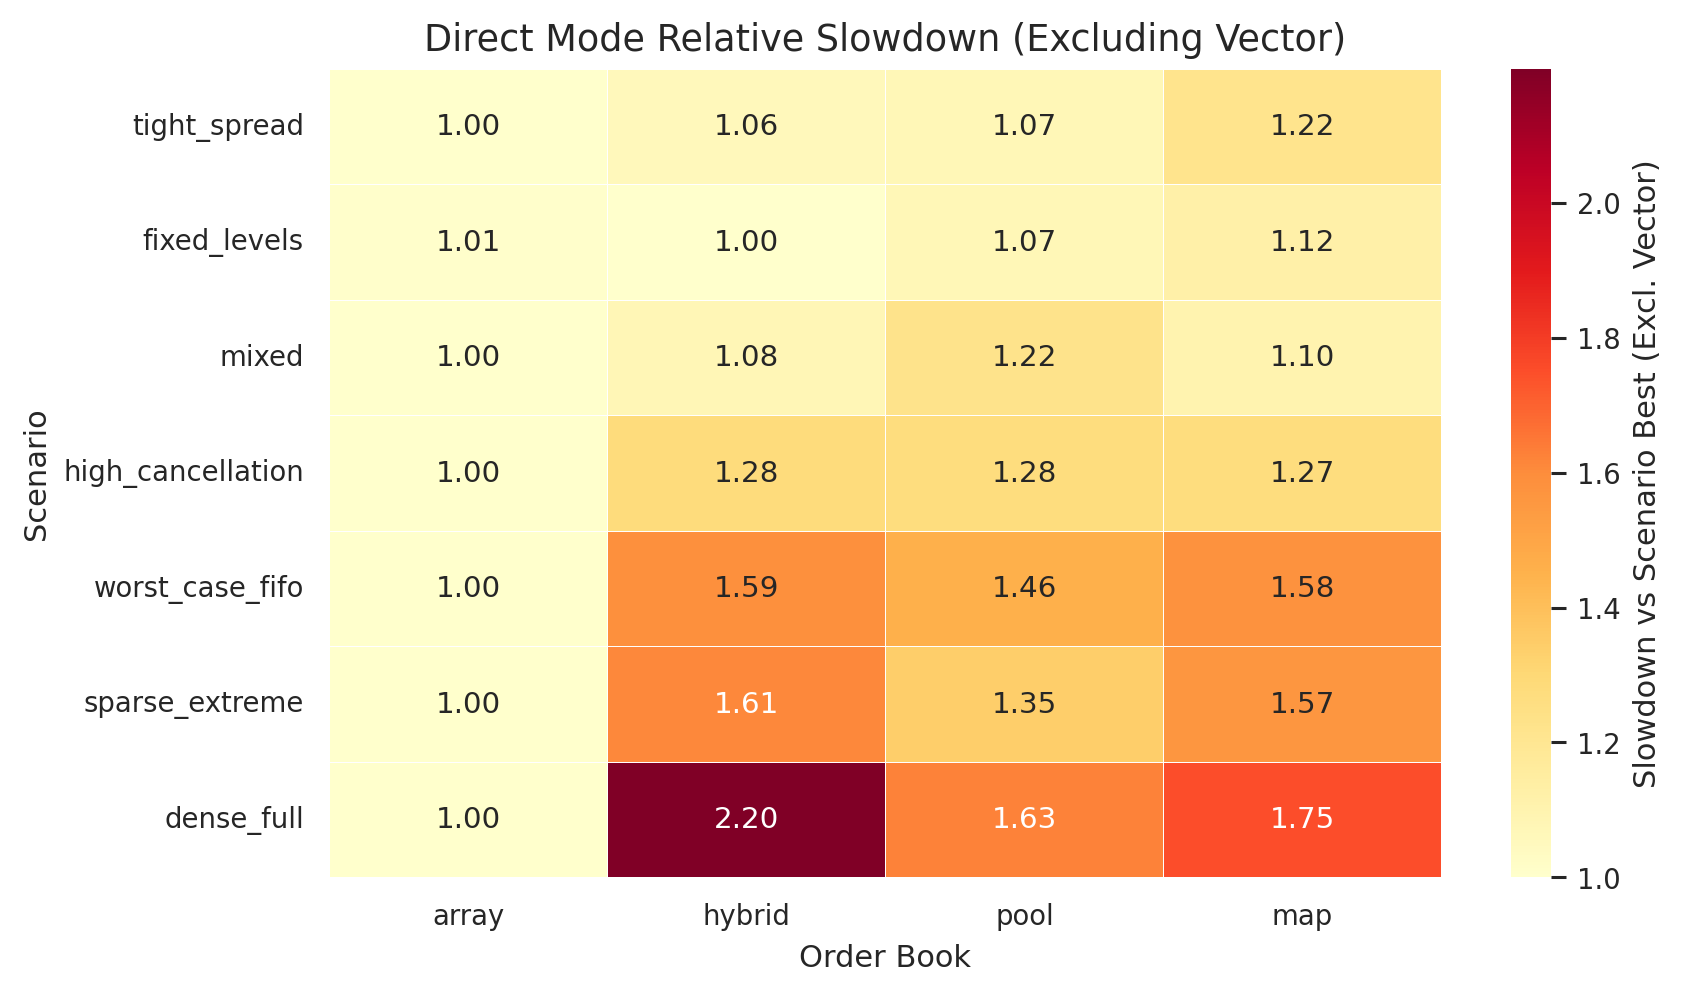
\includegraphics[width=0.8\textwidth]{../plots/direct/latency_slowdown_no_vector_heatmap.png}
    \caption{Direct-mode relative slowdown versus scenario winner (excluding 
    vector). By removing the vector outlier, the performance nuances between the 
    competitive non-vector implementations (Array, Hybrid, Pool, and Map) are 
    preserved in the colormap scale.}
    \label{fig:latency_slowdown_vs_best_heatmap}
\end{figure}

To complement the mean-latency view with dispersion evidence, Figure~\ref{fig:latency_stddev_no_vector_heatmap}
summarises the standard deviation across non-vector implementations in direct mode.
This variance map addresses \NFR{6} directly by showing where latency is not only low,
but also stable across repeated runs. The compact low-variance regions in
\texttt{tight\_spread} and \texttt{fixed\_levels} support the determinism claims made
for array and hybrid layouts, while deeper scenarios show broader spread,
consistent with increased structural and branching pressure.

\begin{figure}[H]
    \centering
    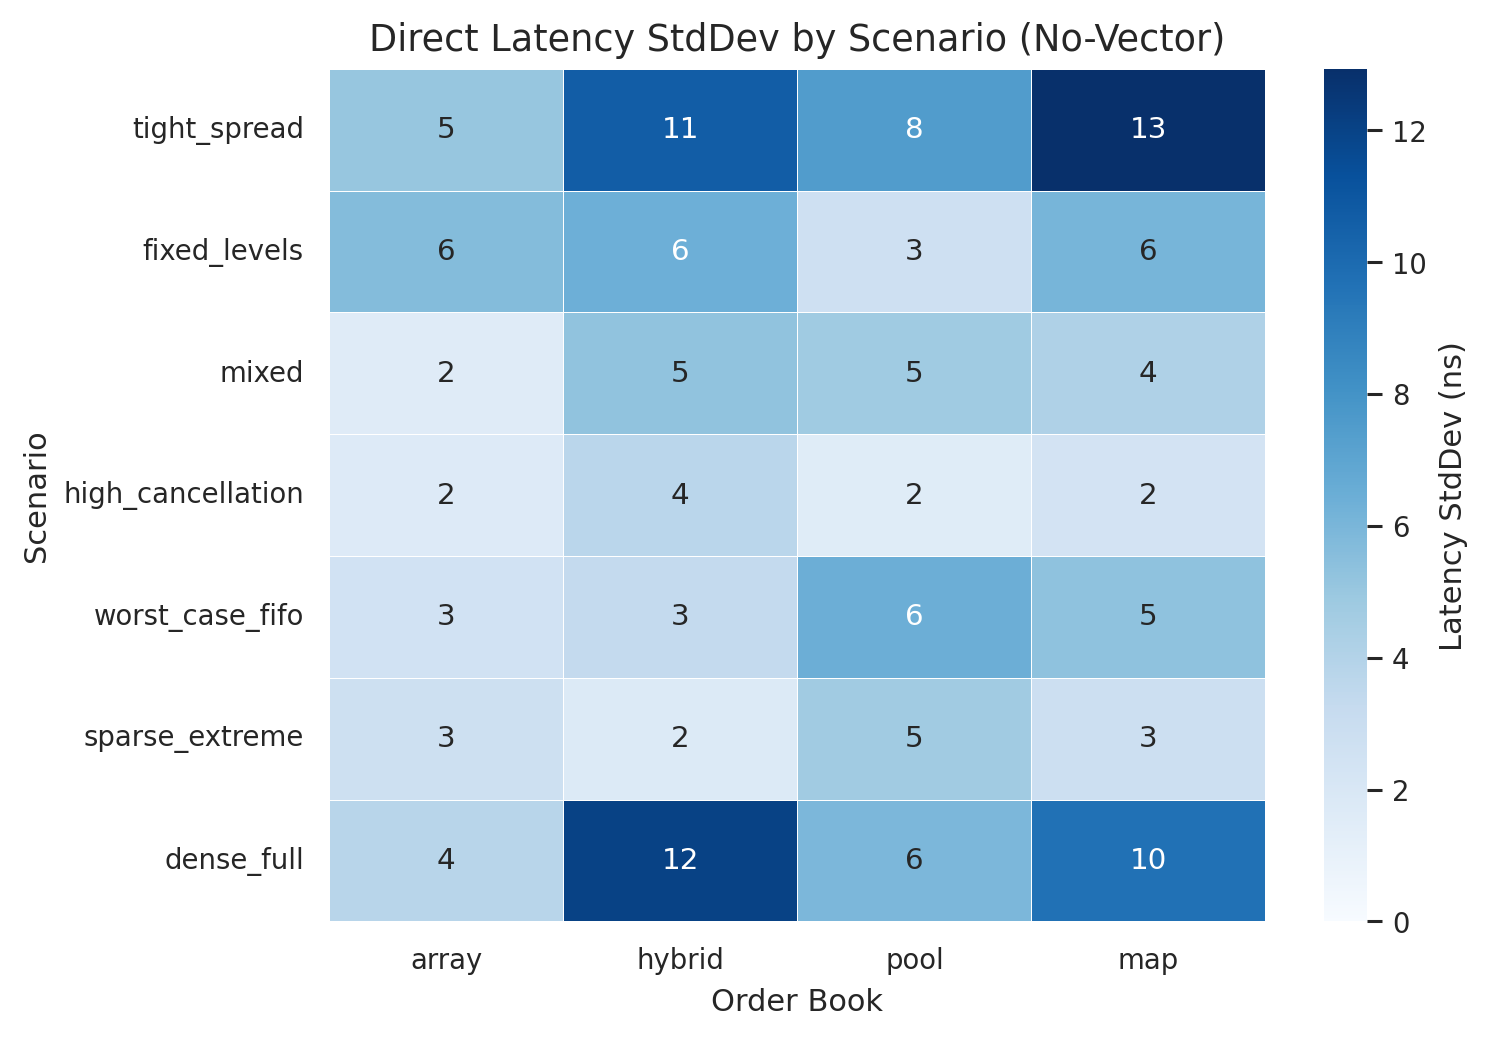
\includegraphics[width=0.8\textwidth]{../plots/direct/latency_stddev_no_vector_heatmap.png}
    \caption{Direct-mode standard-deviation heatmap (excluding vector). Lower 
    values indicate tighter run-to-run stability, providing variance evidence 
    alongside mean latency for \NFR{6}.}
    \label{fig:latency_stddev_no_vector_heatmap}
\end{figure}

\subsection{Architectural Mechanisms: Pool and Hybrid}
\label{subsec:pool_hybrid_mech}
Two novel implementations, the \textbf{HybridOrderBook} and the \textbf{PoolOrderBook},
were engineered in an attempt to mitigate the architectural limitations of the standard
data structures. Rather than relying on a single collection type, these order books employ
more complex internal logic to optimize for specific hardware characteristics.

The \textbf{HybridOrderBook} acts as a substantial improvement over the standard map by
utilizing a tiered architecture: a highly optimized "hot storage" and a slower
"cold storage." It aims to achieve the unbounded flexibility of a map - removing the
strict price-range limitations of the array - while mimicking array-like performance
for the most actively traded prices. The hot storage is implemented as a
capacity-bounded \texttt{std::vector} capped at the top 20 price levels. Because the
vector never exceeds 20 elements, memory-shifting during insertions is practically
instantaneous and fits entirely within the L1 cache. The data supports this
design trade-off. As seen in Table~\ref{tab:direct_mean_latency}, the Hybrid book
achieves a lookup latency of 12.2~ns, exactly matching the
\textbf{ArrayOrderBook}. However, its performance is sensitive to market depth.
In shallow scenarios it is very fast, but in the \texttt{dense\_full} scenario
its mean latency degrades to 208.30~ns. As market depth expands, a majority of orders
are pushed out of the 20-level vector and into the slower cold \texttt{std::map},
subjecting them to tree-traversal overhead.

In contrast, the \textbf{PoolOrderBook} was designed for mechanical sympathy via
pre-allocated nodes, intending to eliminate dynamic heap allocations on the critical path.
While its 17.5~ns insert latency is faster than the map (20.7~ns), it is still slower 
than the array (13.9~ns). It also shows a high match latency of 29.1~ns. 
The \texttt{perf} results show that the logic to manage the free-pool causes a 
7.36\% branch miss rate in the \texttt{mixed} scenario. This penalty is caused 
by the unpredictable "filling logic" in the matching cycle 
(Figure~\ref{fig:pool_match_flow} and Appendix~\ref{app:pool_branching}). 
In a mixed workload, order sizes vary significantly, which prevents the CPU 
from predicting if a match will result in a full or partial fill. As 
illustrated in Figure~\ref{fig:pool_match_flow}, when an order is fully 
consumed, the book must execute a complex path to remove the node and update 
the free-pool. If the fill is partial, this path is skipped. These outcomes in 
the \texttt{mixed} scenario occur with approximately equal frequency, leading 
to branch mispredictions that stall the CPU pipeline~\citep{fog_microarchitecture}.

\begin{figure}[htbp]
    \centering
    \resizebox{0.92\textwidth}{!}{\begin{tikzpicture}[
    node distance=1.5cm and 2cm,
    process/.style={rectangle, minimum width=3cm, minimum height=1cm, text centered, draw=black, fill=blue!10},
    decision/.style={diamond, minimum width=3cm, minimum height=1cm, text centered, draw=black, fill=yellow!20},
    expensive/.style={rectangle, minimum width=3cm, minimum height=1cm, text centered, draw=red, fill=red!10, line width=1pt},
    arrow/.style={thick,->,>=stealth}
]

% Nodes
\node (start) [process] {Calculate Match Quantity};
\node (fill_check) [decision, below=of start] {Order Fully Filled?};

% Branching out
\node (partial) [process, below left=of fill_check, xshift=-0.5cm] {Update Order Quantity};
\node (full) [expensive, below right=of fill_check, xshift=0.5cm] {Remove Node + Return to Pool};

% Join
\node (end) [process, below=2.5cm of fill_check] {Continue Matching};

% Connections
\draw [arrow] (start) -- (fill_check);
\draw [arrow] (fill_check) -| node[anchor=south east, xshift=-0.5cm] {No (Partial)} (partial);
\draw [arrow] (fill_check) -| node[anchor=south west, xshift=0.5cm] {Yes (Full)} (full);
\draw [arrow] (partial) |- (end);
\draw [arrow] (full) |- (end);

% Annotations
\node (prob) [text width=4cm, text centered, font=\small\itshape, right=0.8cm of full, yshift=-0.5cm] 
    {Mixed Scenario:\\$\sim$50\% Probability\\$\implies$ \textbf{Branch Miss}};

\draw [dashed, gray] ($(partial.north west)+(-0.2,0.2)$ ) rectangle ($(full.south east)+(0.2,-0.2)$ );
\node [anchor=north west, font=\footnotesize, gray] at ($(partial.north west)+(-0.2,0.5)$ ) {Divergent Execution Paths};

\end{tikzpicture}
}
    \caption{PoolOrderBook Matching Logic: Divergent Execution Paths}
    \label{fig:pool_match_flow}
\end{figure}

The relative slowdown trends reinforce these architectural trade-offs. 
The \textbf{HybridOrderBook} works well in concentrated markets like 
\texttt{tight\_spread} (126.95~ns) and \texttt{fixed\_levels} (103.39~ns). 
In these scenarios, it outpaces the map by 13.2\% and 11.1\% respectively. 
However, a tier-management penalty appears in the \texttt{dense\_full} scenario, 
where the hybrid is 25.6\% slower than the map. This suggests that managing multiple 
tiers only helps when the top levels are active enough to cover the extra lookup 
costs.

Similarly, the \textbf{PoolOrderBook} shows its advantage in difficult, 
high-memory-pressure scenarios. In \texttt{sparse\_extreme} and 
\texttt{dense\_full}, it outperforms the map by 12.8\% (126.98~ns) and 7.1\% 
(154.02~ns). This performance lead in dispersed layouts highlights the benefit 
of using contiguous memory nodes. These nodes avoid the pointer-chasing and 
allocation costs that slow down the tree-based map. As noted, the book loses 
this advantage in the \texttt{mixed} scenario (112.48~ns vs 100.97~ns) because 
the increased branching penalty outweighs the gains from memory locality.


\begin{table}[htbp]
    \centering
    \small
    \begin{tabular}{lrrrr}
        \toprule
        \textbf{Implementation} & \textbf{Insert (ns)} & \textbf{Cancel (ns)} & \textbf{Lookup (ns)} & \textbf{Match (ns)} \\
        \midrule
        ArrayOrderBook   & 13.9 & 12.2 & 12.2 & 14.2 \\
        MapOrderBook     & 20.7 & 23.8 & 13.0 & 14.7 \\
        VectorOrderBook  & 20.9 & 22.3 & 12.8 & 14.1 \\
        HybridOrderBook  & 20.9 & 22.5 & 12.2 & 13.9 \\
        PoolOrderBook    & 17.5 & 23.2 & 12.6 & 29.1 \\
        \bottomrule
    \end{tabular}
    \caption{Mean Operation Latency in Direct Mode (nanoseconds)}
    \label{tab:direct_mean_latency}
\end{table}

Figure~\ref{fig:mixed_operation_breakdown} provides a granular cost 
decomposition of the \texttt{mixed} scenario, revealing the specific 
operational trade-offs behind these architectural trends. The 
\texttt{HybridOrderBook} achieves its performance lead through lower 
\texttt{Lookup} and \texttt{Insert} latencies compared to the map, 
validating the efficacy of its "hot storage" layer. Conversely, the 
\texttt{PoolOrderBook} is dragged down by its \texttt{Match} operation, which 
is consistently slower than the map (29.1~ns vs 14.7~ns) due to the branching 
penalty discussed. This data confirms that while memory locality helps in 
dense markets, the logical complexity of managing a pool can become the 
dominant bottleneck in standard trading workloads.


\begin{figure}[htbp]
    \centering
    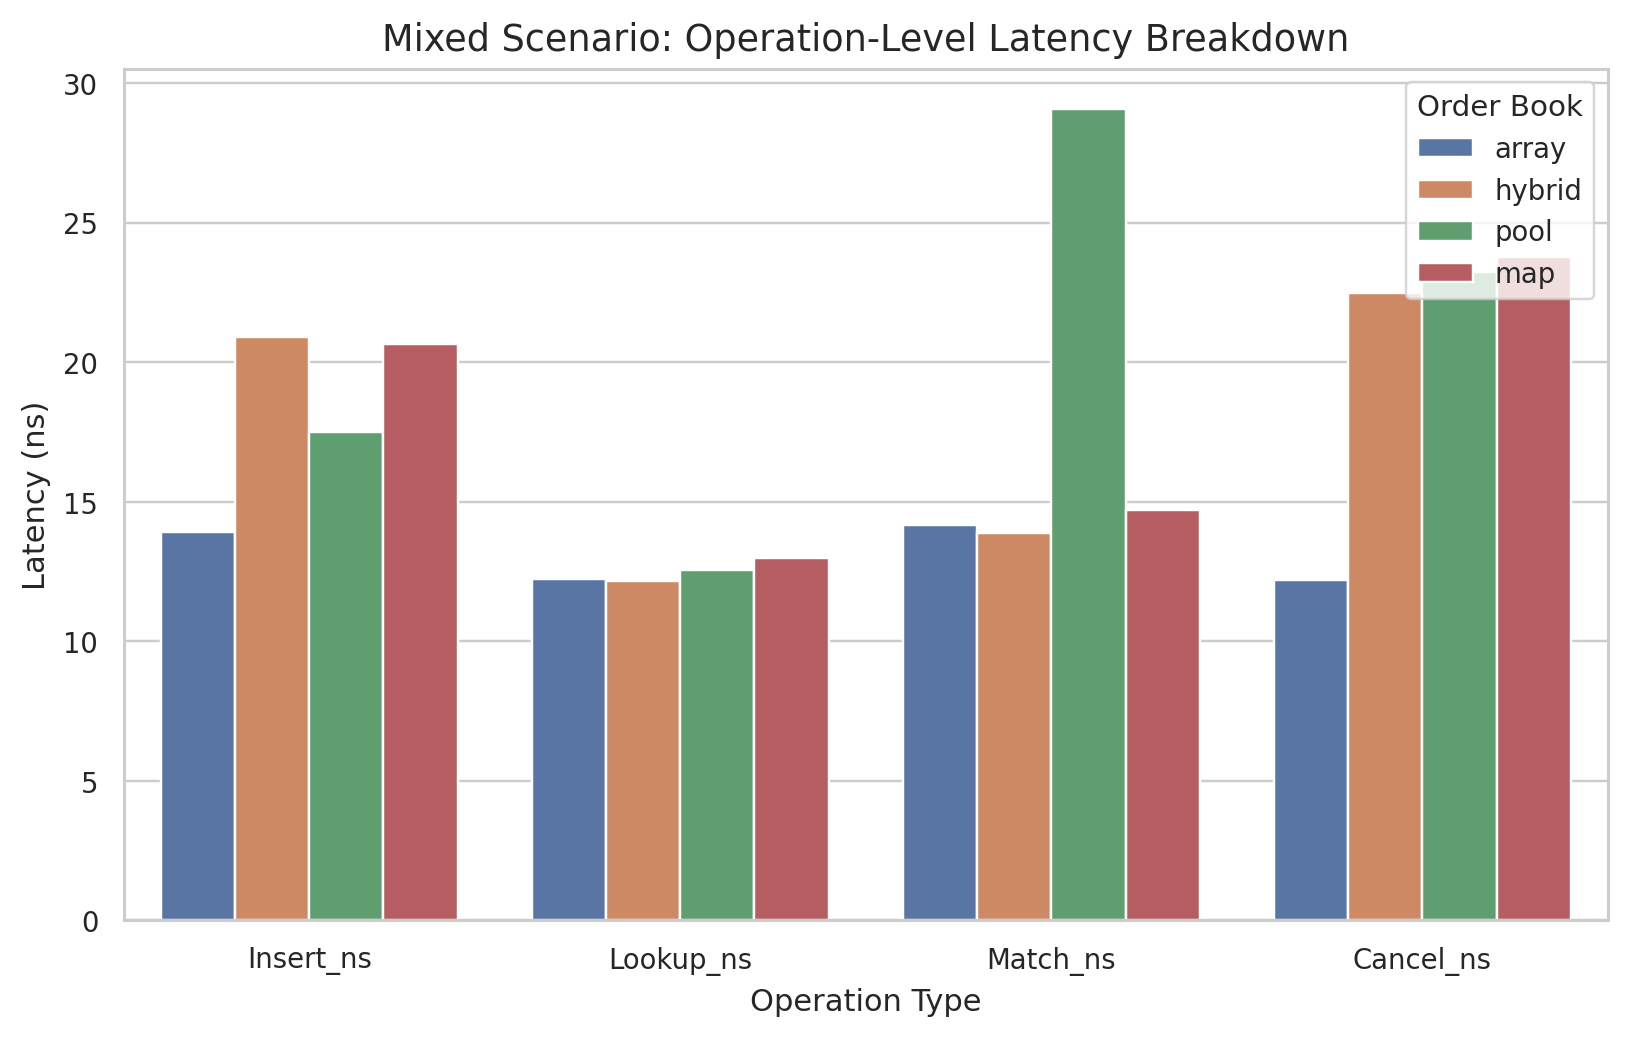
\includegraphics[width=0.8\textwidth]{../plots/direct/mixed_operation_latency_breakdown.png}
    \caption{Cost decomposition of the \texttt{mixed} scenario (direct mode). The 
    comparison highlights the Hybrid book's advantage in lookups and the Pool's 
    match-processing bottleneck.}
    \label{fig:mixed_operation_breakdown}
\end{figure}

\paragraph{Architectural Selection: No Universal Answer.}
The evidence gathered here shows that no single order book is the best choice
for every market.
Each implementation performs well under particular workload conditions and
poorly under others.
This finding has a direct practical consequence: the optimal data structure
for a given exchange is a function of that exchange's market conditions, not
an engineering absolute.
If an operator can model their expected order flow - for example through
historical data collection or Monte Carlo simulation of order arrivals, fill
rates, and cancellation frequency - they can match the implementation to
the workload.
For a venue similar to a \textbf{NASDAQ equity market}, where tick-constrained
stocks concentrate activity at a small number of near-spread price levels
\citep{harris1994minimum}, both the \texttt{ArrayOrderBook} and the
\texttt{HybridOrderBook} are strong candidates.
The array's \texttt{tight\_spread} latency of 91.72~ns and the hybrid's
advantage in \texttt{fixed\_levels} (103.39~ns, 11.1\% faster than the map)
reflect this well.
In contrast, a venue resembling a \textbf{CME E-mini futures} market, where
order flow is sparse across many price levels and institutional orders arrive
with large, unpredictable sizes, would favour the \texttt{PoolOrderBook} or
\texttt{MapOrderBook} over the array, since the latter's fixed interval
requires all valid prices to be pre-allocated, making rebalancing expensive
when price ranges shift rapidly~\citep{gould2013lob}.
The \texttt{ArrayOrderBook}'s inflexibility is also a concern for venues
where participants expect continuous price freedom without tick constraints.
If a client wishes to bid or ask at any arbitrary price, the array's
pre-allocated, integer-indexed structure may impose a structural limitation
that is unacceptable in practice.
Holistically, as market conditions are dynamic and exchanges serve participants
with different objectives, there is no universally correct order book.
The right approach is to treat data structure selection as an empirical
decision, driven by workload profiling and the trade-offs identified here.

\subsection{Tail Latency Distribution and Determinism}
\label{subsec:tail_latency}
Beyond mean performance, a critical metric for evaluating a high-frequency trading 
system is the \textbf{P99 tail latency}. 
This represents the performance of the bottom 1\% of operations captured over a 
benchmark duration. 
In the zero-sum competitive environment of HFT, these worst-case outliers often 
represent the difference between a profitable execution and a severe 
financial loss. 
A single high-latency event during a period of extreme market volatility can result 
in missed liquidation opportunities or unintended exposure, potentially 
jeopardizing a firm's solvency. 

The primary trend observed in Table~\ref{tab:direct_p99_latency} is that the 
\texttt{ArrayOrderBook} provides the most deterministic performance profile. 
Its P99 latency remains remarkably stable across both \texttt{mixed} (125~ns) 
and \texttt{dense} (133~ns) workloads, demonstrating that increasing book 
complexity does not impact its execution path. 
This stability sets the "gold standard" for \ref{hyp:h2}, indicating that a simpler 
linear layout is inherently more predictable. 
In contrast, every other implementation see its tail latency at least double 
under pressure (comparing 125~ns to thresholds above 300~ns). 

The most significant regression is found in the \texttt{VectorOrderBook}, which 
exhibits a severe tail expansion from 141~ns in \texttt{mixed} to 
6,016~ns in \texttt{dense\_full} (a 42x increase). 
As previously discussed, this behavior is a direct consequence of the 
requirement to continuously shift elements in memory during insertion and 
frequently resize the underlying container, leading to devastating 
performance costs when the book is deep. 

The \texttt{PoolOrderBook} also exhibits a distinct tail profile. 
In the \texttt{mixed} scenario, it performs significantly worse than the 
array (208~ns vs 125~ns) due to the high frequency of branch mispredictions 
documented in Section~\ref{subsec:pool_hybrid_mech}. 
This data provides a direct validation of \ref{hyp:h2}: although memory 
pooling reduces allocation jitter, it cannot overcome the fundamental 
performance bottlenecks (in this case, branching stalls) of a more 
logically complex data structure. 
However, in the \texttt{dense\_full} case, the pool's P99 improves relative 
to the map-based books (308~ns vs 383~ns for the Map). 
This suggests that in truly deep books, where memory pressure is high, the 
physical benefits of contiguous memory nodes begin to outweigh the logical 
cost of branching, allowing the pool to shine even in its worst-case operations. 

Finally, the \texttt{HybridOrderBook} exhibits a performance ceiling in deep 
markets. 
While its tail is competitive in \texttt{mixed} (141~ns), it is beaten by the 
standard map in the \texttt{dense\_full} scenario (491~ns vs 383~ns). 
This is because in a 2,000-level book, the "hot storage" (limited to the top 20 
levels) is almost always exhausted, forcing the system to pay a dual tax: 
the overhead of checking the hot-tier followed by a full tree traversal in the 
cold-tier.



\begin{table}[htbp]
    \centering
    \small
    \begin{tabular}{lrr}
        \toprule
        \textbf{Implementation} & \textbf{P99 Mixed (ns)} & \textbf{P99 Dense (ns)} \\
        \midrule
        ArrayOrderBook   & 125 & 133 \\
        MapOrderBook     & 150 & 383 \\
        VectorOrderBook  & 141 & 6,016 \\
        HybridOrderBook  & 141 & 491 \\
        PoolOrderBook    & 208 & 308 \\
        \bottomrule
    \end{tabular}
    \caption{P99 Tail Latency in Direct Mode (nanoseconds)}
    \label{tab:direct_p99_latency}
\end{table}

\begin{figure}[htbp]
    \centering
    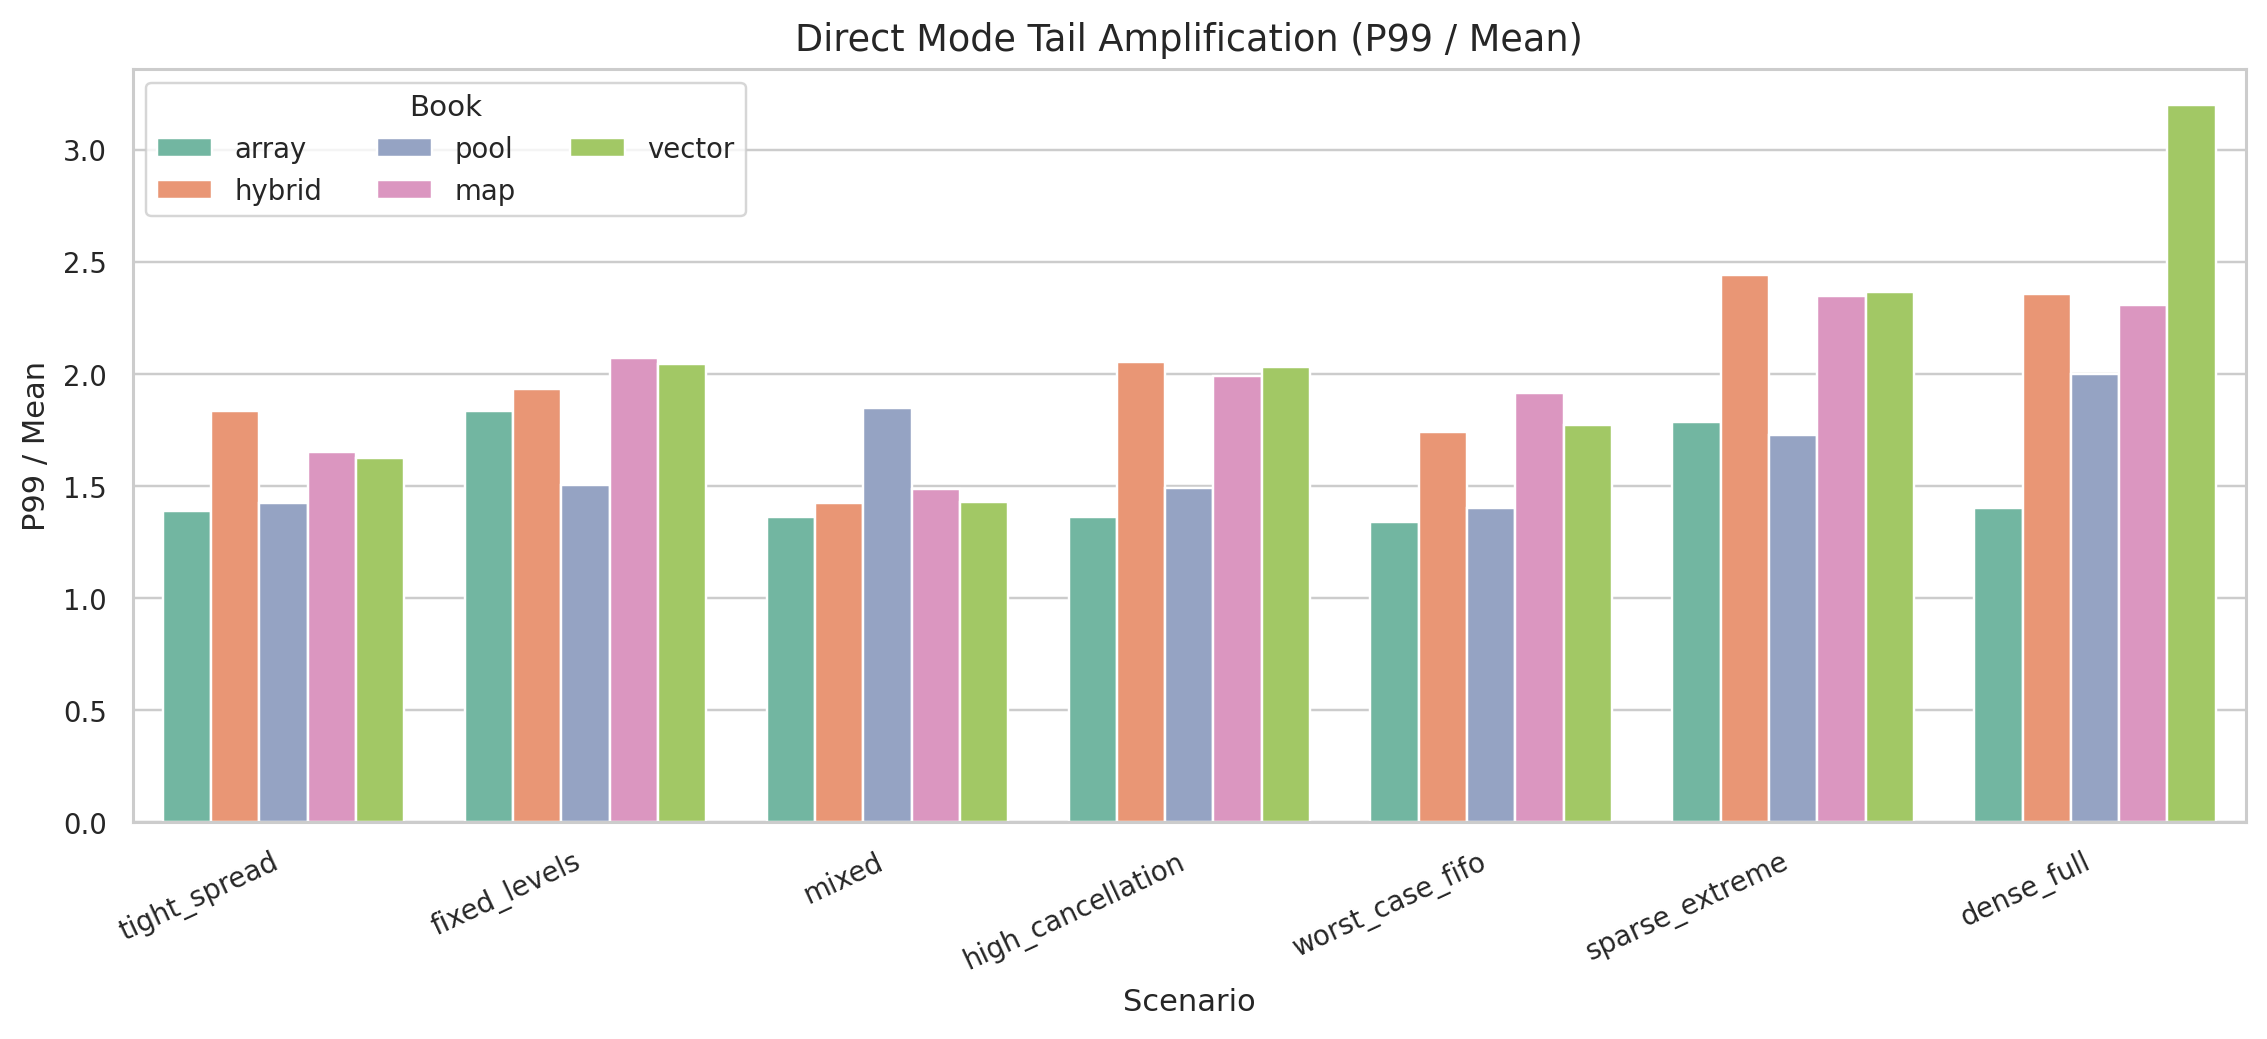
\includegraphics[width=0.8\textwidth]{../plots/direct/tail_p99_over_mean.png}
    \caption{Tail inflation map using P99-to-mean ratio in direct mode. Several 
    map and vector cases exhibit elevated tail amplification relative to mean 
    latency, indicating sensitivity to jitter and/or burst conditions.}
    \label{fig:tail_p99_over_mean}
\end{figure}

The cumulative data from direct mode testing strongly supports both \ref{hyp:h1} 
and \ref{hyp:h2}. 
The \texttt{ArrayOrderBook} consistently delivered the highest throughput and 
the lowest mean latency across almost all market scenarios. 
Its ability to maintain a tight P99 tail latency under load confirms that 
index-based, cache-friendly layouts are inherently faster and more deterministic 
than complex data structures. 
Conversely, the data supports \ref{hyp:h2} by showing that while the 
\texttt{PoolOrderBook} improved upon the \texttt{MapOrderBook} in specific 
high-density scenarios through contiguous memory, it could not match the array. 
The branching penalties required to manage the memory pool created a firm 
performance ceiling. 
Therefore, we accept both hypotheses: direct array indexing is the superior 
method for algorithmic matching, and memory pooling is an optimization rather 
than a fundamental solution to data structure complexity.

\section{Gateway Mode - End-to-End Decomposition}

To evaluate \ref{hyp:h3} (System-Level Masking), the benchmark transitioned from 
direct isolated execution to a fully networked Gateway mode. 
This mode simulates a realistic exchange architecture, where orders travel 
from a client over a TCP socket, are parsed from FIX messages, passed through 
a lock-free SPSC queue, and finally processed by the matching engine. 
To accurately identify bottlenecks across this pipeline, a "triple-timestamp" 
telemetry system was implemented (illustrated in Figure~\ref{fig:telemetry_pipeline}). 
Four exact timestamps are recorded for every order: the client capture before 
writing to the socket ($T_1$), the gateway capture upon 
receiving and parsing the message into a C++ struct ($T_2$), the engine capture 
immediately after dequeuing ($T_3$), and the final completion 
capture ($T_4$). 
By calculating the deltas between these timers, total end-to-end latency is 
decomposed into three strict buckets:
\begin{itemize}
    \item \textbf{Network (Net):} The time taken to traverse the TCP socket, the 
    operating system stack, and decode the FIX payload (\texttt{T2 - T1}).
    \item \textbf{Queue (Que):} The time spent waiting in the thread-handoff lock-free queue (\texttt{T3 - T2}).
    \item \textbf{Engine (Eng):} The pure algorithmic latency consumed by the order book logic (\texttt{T4 - T3}).
\end{itemize}

\begin{figure}[H]
    \centering
    \resizebox{0.92\textwidth}{!}{\begin{tikzpicture}[
    node distance=2.8cm,
    block/.style={rectangle, draw, fill=blue!5, text width=2.4cm, text centered, rounded corners, minimum height=1.2cm},
    line/.style={draw, -latex', thick},
    timer/.style={circle, draw, fill=red!10, inner sep=1pt, font=\small\bfseries}
]

% Nodes
\node [block] (client) {Gateway Client};
\node [block, right=of client] (gateway) {TCP Gateway \& FIX Parser};
\node [block, right=of gateway] (queue) {Lock-Free SPSC Queue};
\node [block, right=of queue] (engine) {Matching Engine};

% Arrows
\path [line] (client) -- node[above] {TCP/IP} (gateway);
\path [line] (gateway) -- node[above] {Push} (queue);
\path [line] (queue) -- node[above] {Pop} (engine);

% Timers overlay
\node [timer] at ($(client.east) + (0.3, 0.4)$) (t1) {$T_1$};
\node [timer] at ($(gateway.east) + (0.3, 0.4)$) (t2) {$T_2$};
\node [timer] at ($(queue.east) + (0.3, 0.4)$) (t3) {$T_3$};
\node [timer] at ($(engine.east) + (0.3, 0.4)$) (t4) {$T_4$};

% Specific timestamp labels
\node [align=left, font=\scriptsize, anchor=south, yshift=0.2cm] at (t1.north) {\texttt{sendTimestamp}\\(Before socket write)};
\node [align=left, font=\scriptsize, anchor=south, yshift=0.2cm] at (t2.north) {\texttt{receiveTimestamp}\\(After struct parse)};
\node [align=left, font=\scriptsize, anchor=south, yshift=0.2cm] at (t3.north) {\texttt{engineStart}\\(After queue pop)};
\node [align=left, font=\scriptsize, anchor=south, yshift=0.2cm] at (t4.north) {\texttt{engineEnd}\\(After match)};

% Labels for buckets
\draw [|-|, thick, blue!80!black] ($(client.east)+(0,-1.5)$) -- node[below, font=\small\bfseries] {Net} ($(gateway.east)+(0,-1.5)$);
\draw [|-|, thick, green!60!black] ($(gateway.east)+(0,-1.5)$) -- node[below, font=\small\bfseries] {Que} ($(queue.east)+(0,-1.5)$);
\draw [|-|, thick, red!80!black] ($(queue.east)+(0,-1.5)$) -- node[below, font=\small\bfseries] {Eng} ($(engine.east)+(0,-1.5)$);

\end{tikzpicture}
}
    \caption{End-to-End Telemetry Checkpoints. The pipeline is instrumented with 
    four precise timestamps to isolate transport, queuing, and matching 
    latencies.}
    \label{fig:telemetry_pipeline}
\end{figure}

\begin{table}[htbp]
    \centering
    \small
    \begin{tabular}{lrrrr}
        \toprule
        \textbf{Implementation} & \textbf{Total (ns)} & \textbf{Net (ns)} & \textbf{Queue (ns)} & \textbf{Engine (ns)} \\
        \midrule
        ArrayOrderBook   & 463,149 & 462,884 &    248 &  16 \\
        MapOrderBook     & 426,402 & 425,980 &    345 &  79 \\
        VectorOrderBook  & 1,008,074 & 784,804 & 229,974 & 300 \\
        HybridOrderBook  & 405,912 & 405,549 &    286 &  77 \\
        PoolOrderBook    & 418,697 & 418,337 &    336 &  55 \\
        \bottomrule
    \end{tabular}
    \caption{End-to-End Latency Decomposition in Gateway Mode (nanoseconds), averaged across all seven scenarios}
    \label{tab:gateway_decomposition}
\end{table}

\begin{figure}[H]
    \centering
    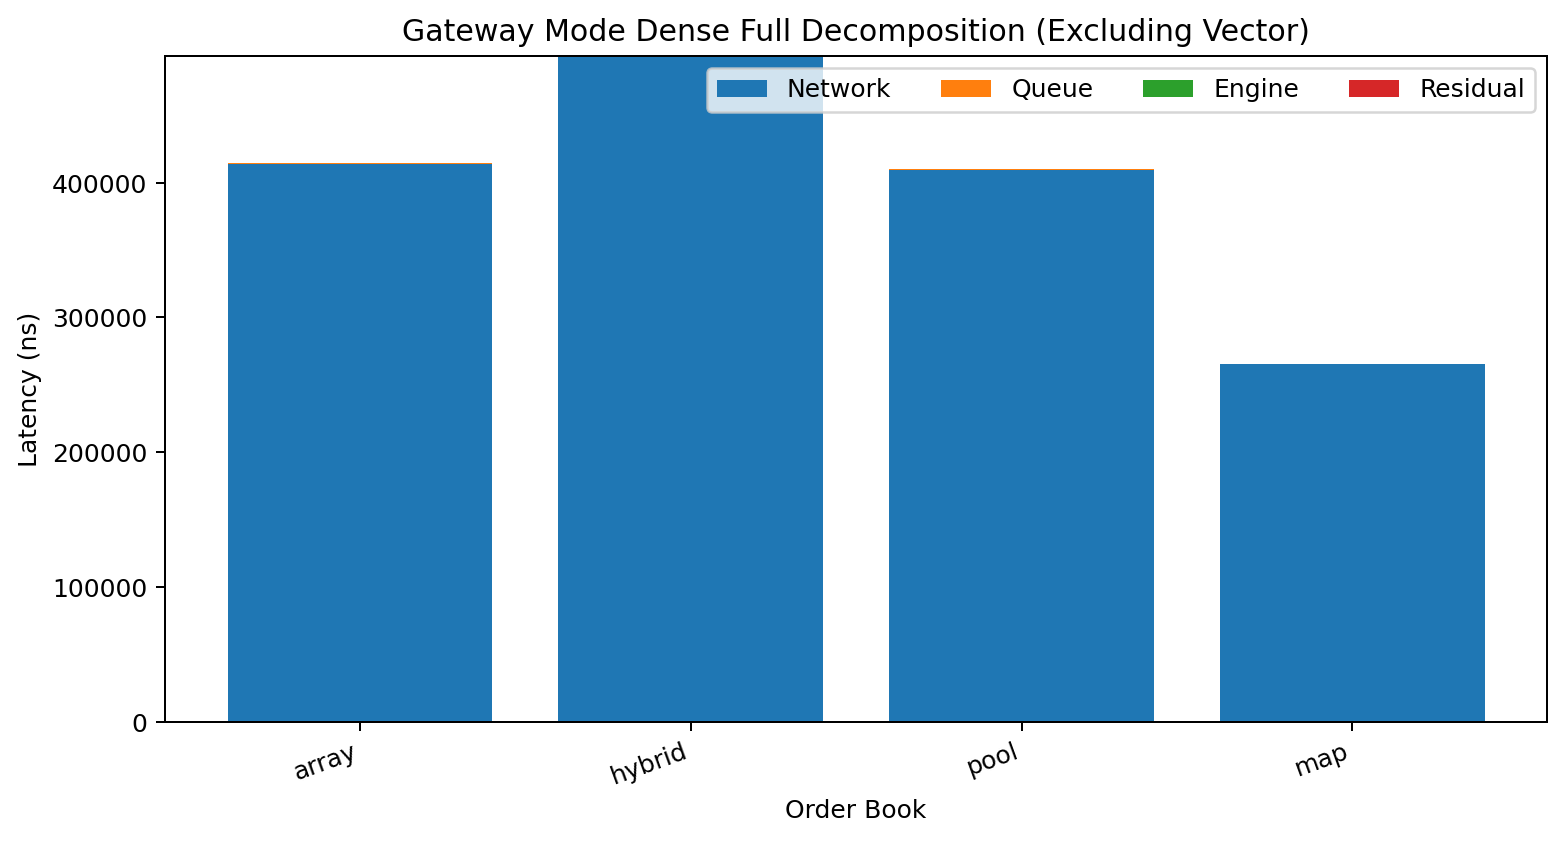
\includegraphics[width=0.8\textwidth]{../plots/gateway/dense_full_latency_decomposition_no_vector.png}
    \caption{Dense\_full gateway decomposition (network, queue, engine) for 
    non-vector implementations. The vector row is omitted in this comparative 
    view because its dense\_full queue and network outlier compresses the 
    non-vector bars.}
    \label{fig:gateway_decomposition}
\end{figure}

As seen in Table~\ref{tab:gateway_decomposition}, the total end-to-end latency is
dominated by the network component.
For a standard implementation like the \texttt{ArrayOrderBook}, the network
accounts for 462,884~ns of the total 463,149~ns.
In contrast, the actual matching engine work takes up only 16~ns.
This indicates that almost all time spent processing an order in gateway
mode is consumed by the Linux network stack and TCP transport.
The data provides clear evidence for \ref{hyp:h3}.
In a realistic networked environment, the nanosecond-level gains achieved
by better order book data structures are substantially masked by the
millisecond-scale jitter of the transport layer.
These gateway-mode findings are consistent with exchange-scale evidence that
small latency advantages can still be economically meaningful under realistic
market conditions~\citep{aquilina2022armsrace}.
This is consistent with the broader tail-latency literature, where
end-to-end variance is often dominated by transport and queueing effects
rather than isolated compute kernels~\citep{dean2013tail}.
Unless the exchange implements kernel-bypass techniques (such as DPDK or Solarflare
OpenOnload)~\citep{redhat2012_openonload}, the choice of order book implementation remains a secondary
concern for overall system latency.
Holistically, while the algorithmic choice is critical for isolating performance,
the system-level bottlenecks define the practical experience for the client.

\begin{figure}[H]
    \centering
    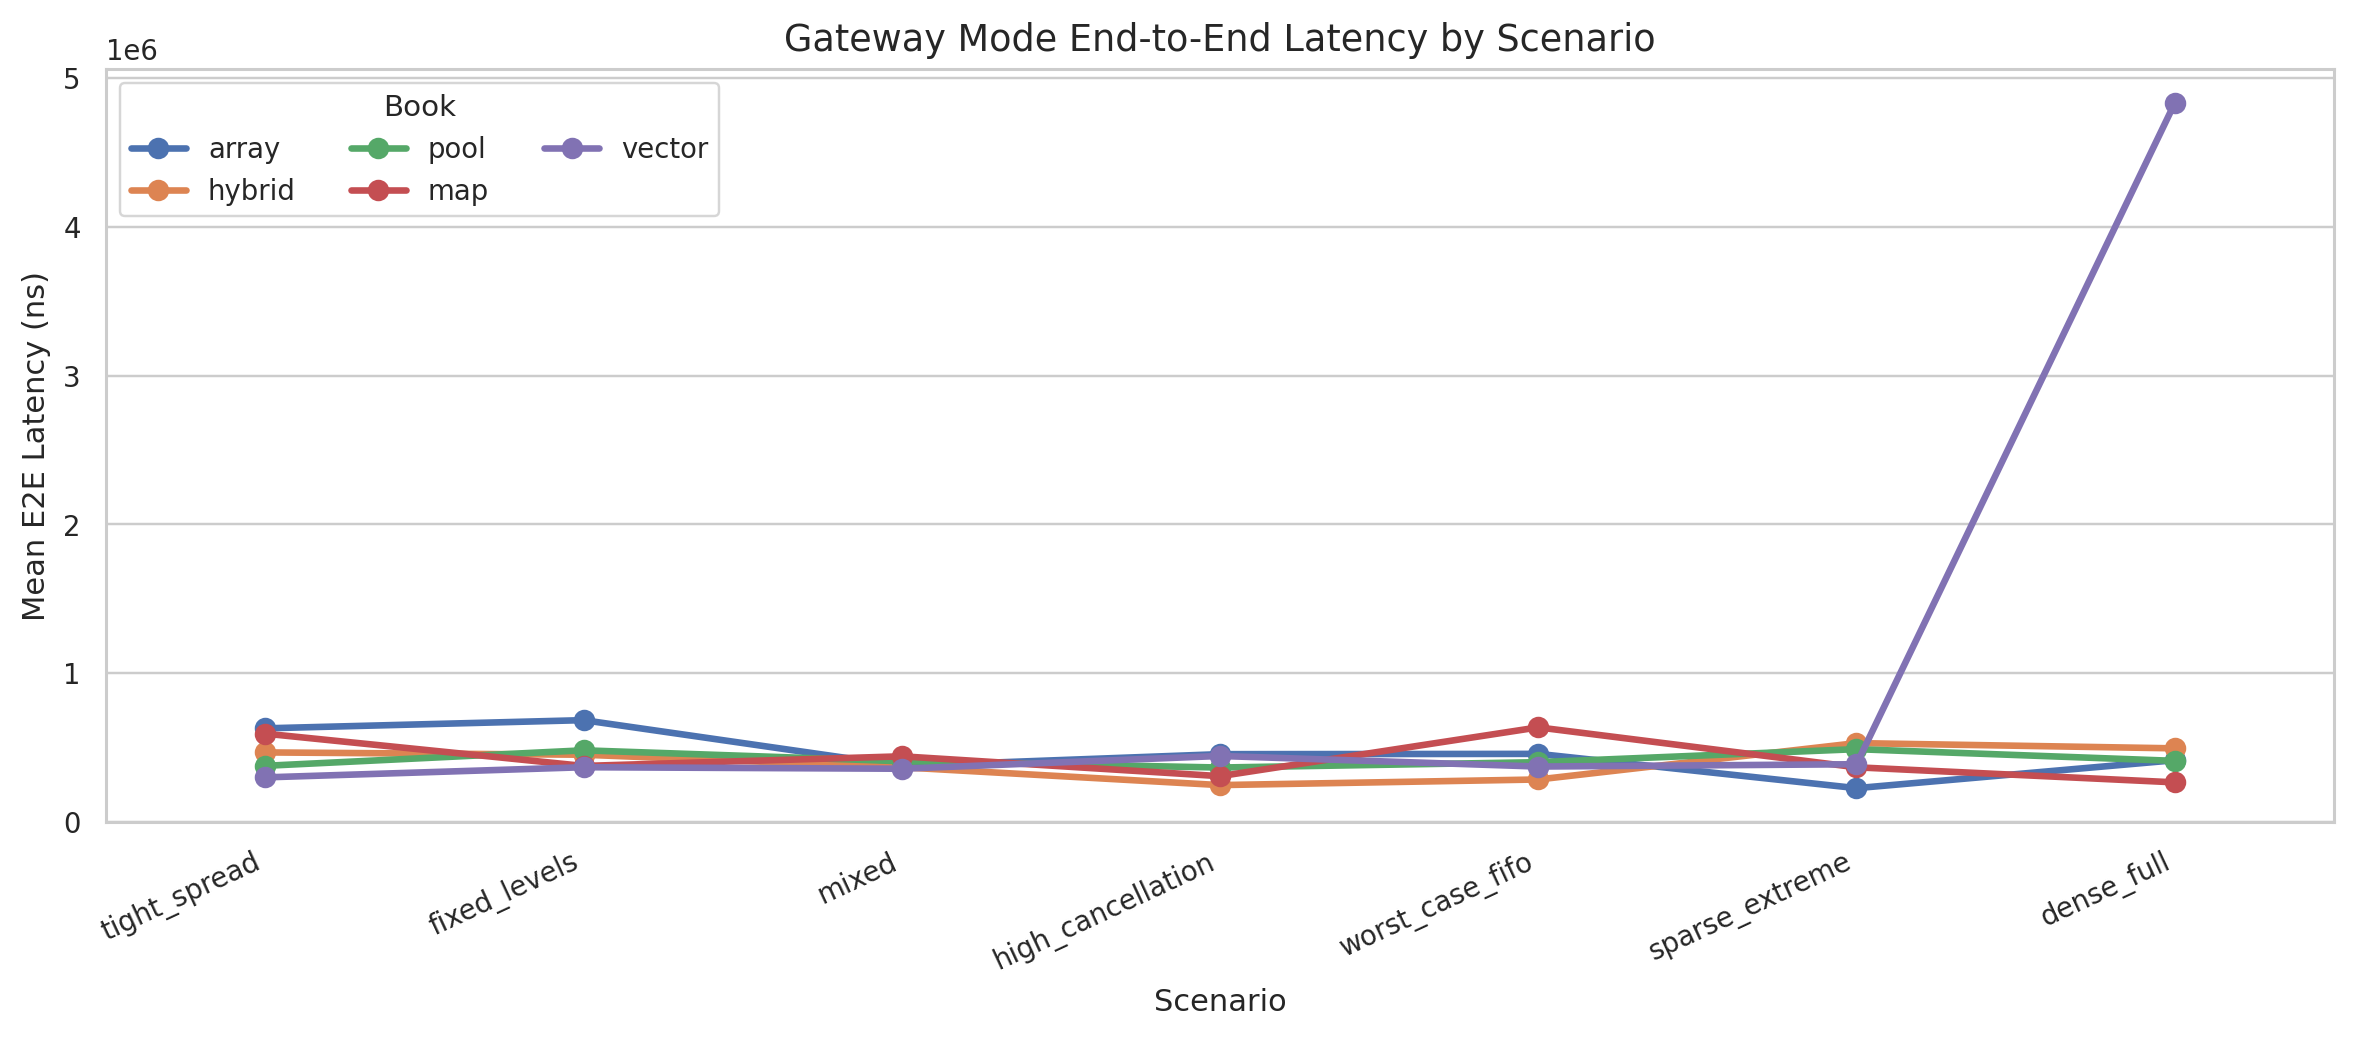
\includegraphics[width=0.8\textwidth]{../plots/gateway/latency_by_scenario.png}
    \caption{Gateway latency by scenario across all implementations. The plot 
    shows mean end-to-end latency patterns only; the masking claim is supported 
    by the decomposition in Table~\ref{tab:gateway_decomposition}.}
    \label{fig:gateway_latency_by_scenario}
\end{figure}

Figure~\ref{fig:gateway_latency_by_scenario} compares mean gateway latency by
scenario across all books.
It is a visual summary, not proof on its own.
The main point is that results move by scenario, but all books are still in the
same broad microsecond range because transport and queue costs dominate.
Table~\ref{tab:gateway_decomposition} and Figure~\ref{fig:gateway_decomposition}
use different scopes: the table is averaged across all scenarios, while the
decomposition figure is dense\_full only.
Outside \texttt{dense\_full} in gateway mode, vector also outperforms map in 
four of six scenarios (\texttt{tight\_spread}, \texttt{fixed\_levels}, 
\texttt{mixed}, and \texttt{worst\_case\_fifo}), which is consistent with the 
scenario plot.
For vector, dense\_full is a major outlier (about 4.83 ms), but the other six
scenarios are around 0.30--0.44 ms, so the all-scenario mean is much lower
(about 1.01 ms).

\section{MPSC Thread Contention} 
\label{sec:mpsc_contention}

To test the system's ability to scale to $n$ concurrent clients, we utilize 
Moody's lock-free MPMC queue in our simulated exchange. 
By generating concurrent load through multiple producer threads, we can analyze 
how the order book handles cross-thread contention over the shared buffer. 
This isolates L3 cache coherence effects from network layer delays, directly 
adhering to the performance isolation mechanisms required by~\NFR{7}.

\begin{figure}[htbp]
    \centering
    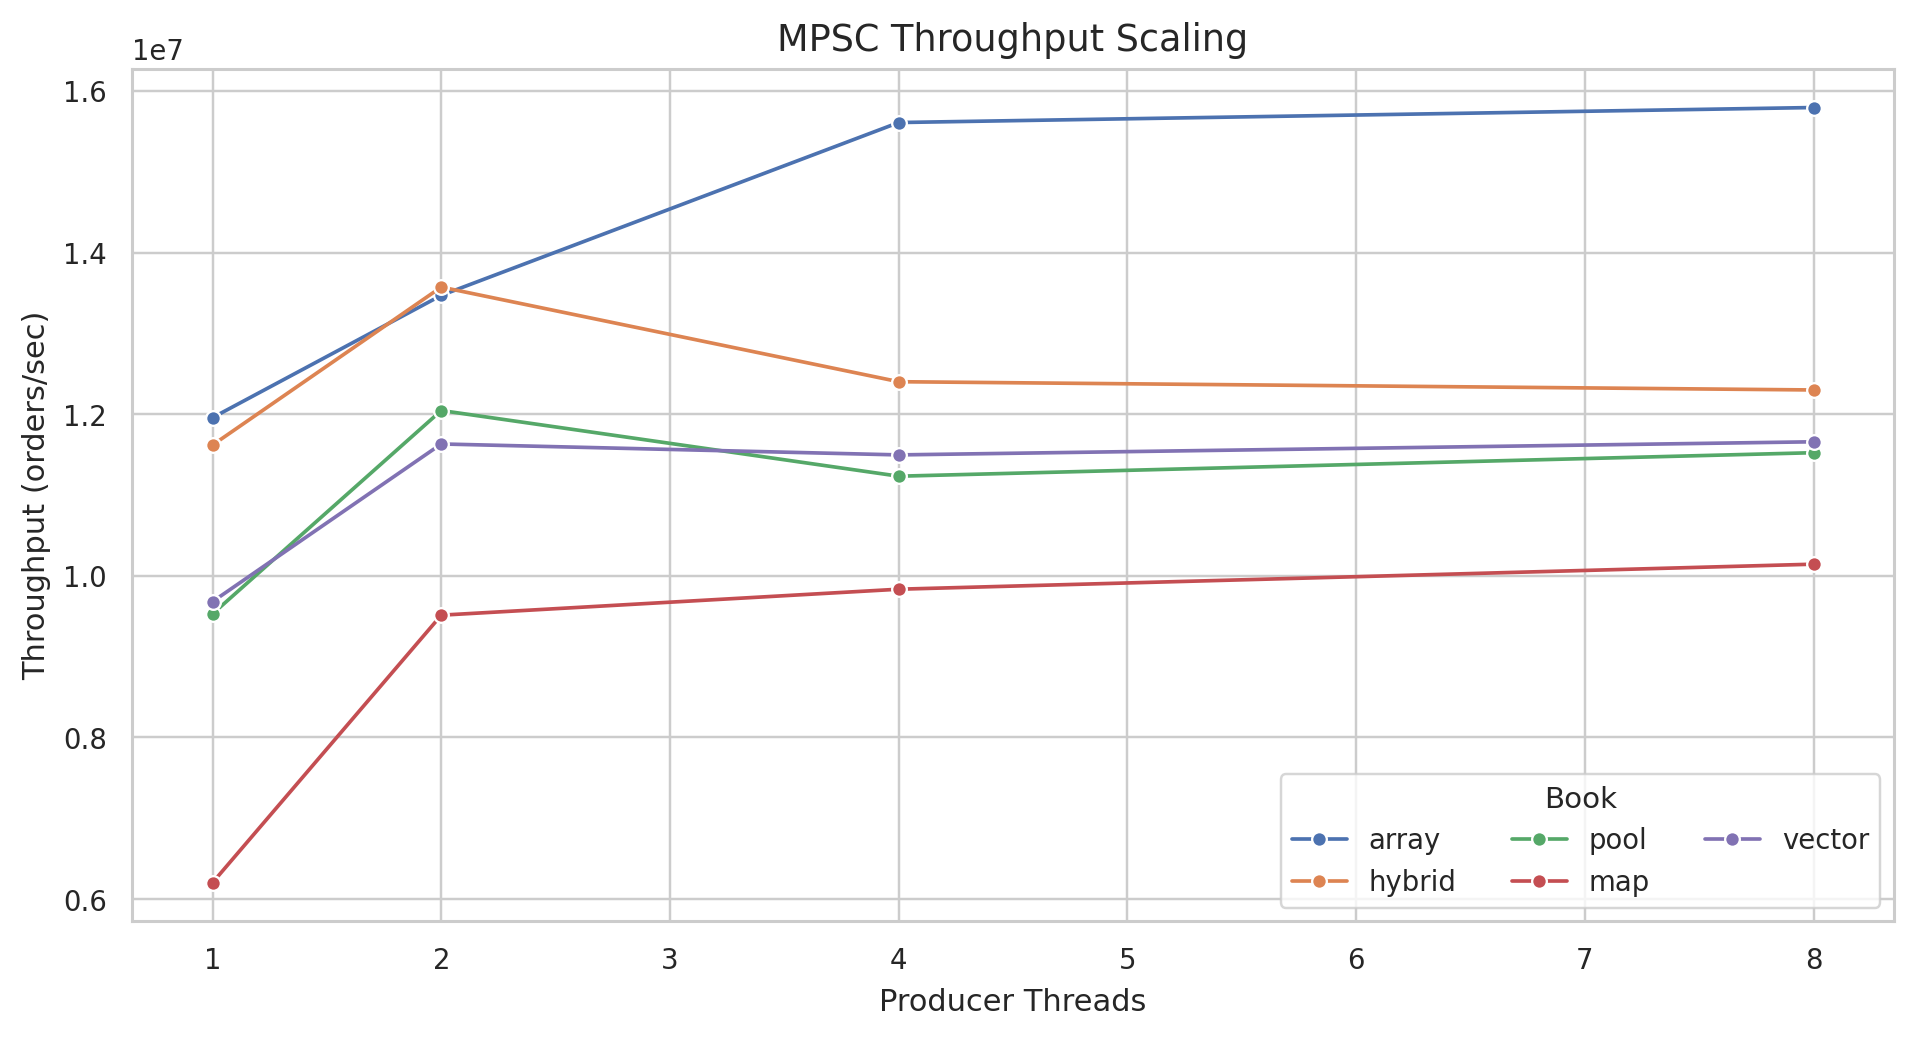
\includegraphics[width=0.8\textwidth]{../plots/mpsc/throughput_scaling.png}
    \caption{Throughput scaling under varying producer thread counts in MPSC 
    mode. Identifies the contention point where the single consumer matching 
    engine becomes the bottleneck.}
    \label{fig:mpsc_throughput}
\end{figure}

As shown in Figure~\ref{fig:mpsc_throughput}, the system throughput 
increases when we move from one producer thread to two. 
However, when we increase the threads to four and eight, the throughput stops 
growing and stays at a flat level for all order books. 
This happens because the single matching engine has reached its absolute working 
limit. 
For example, the array order book hits a maximum speed of about 15.7 million 
operations per second. 
At this point, the engine cannot read orders from the lock-free queue any faster 
than it already is.

\begin{figure}[htbp]
    \centering
    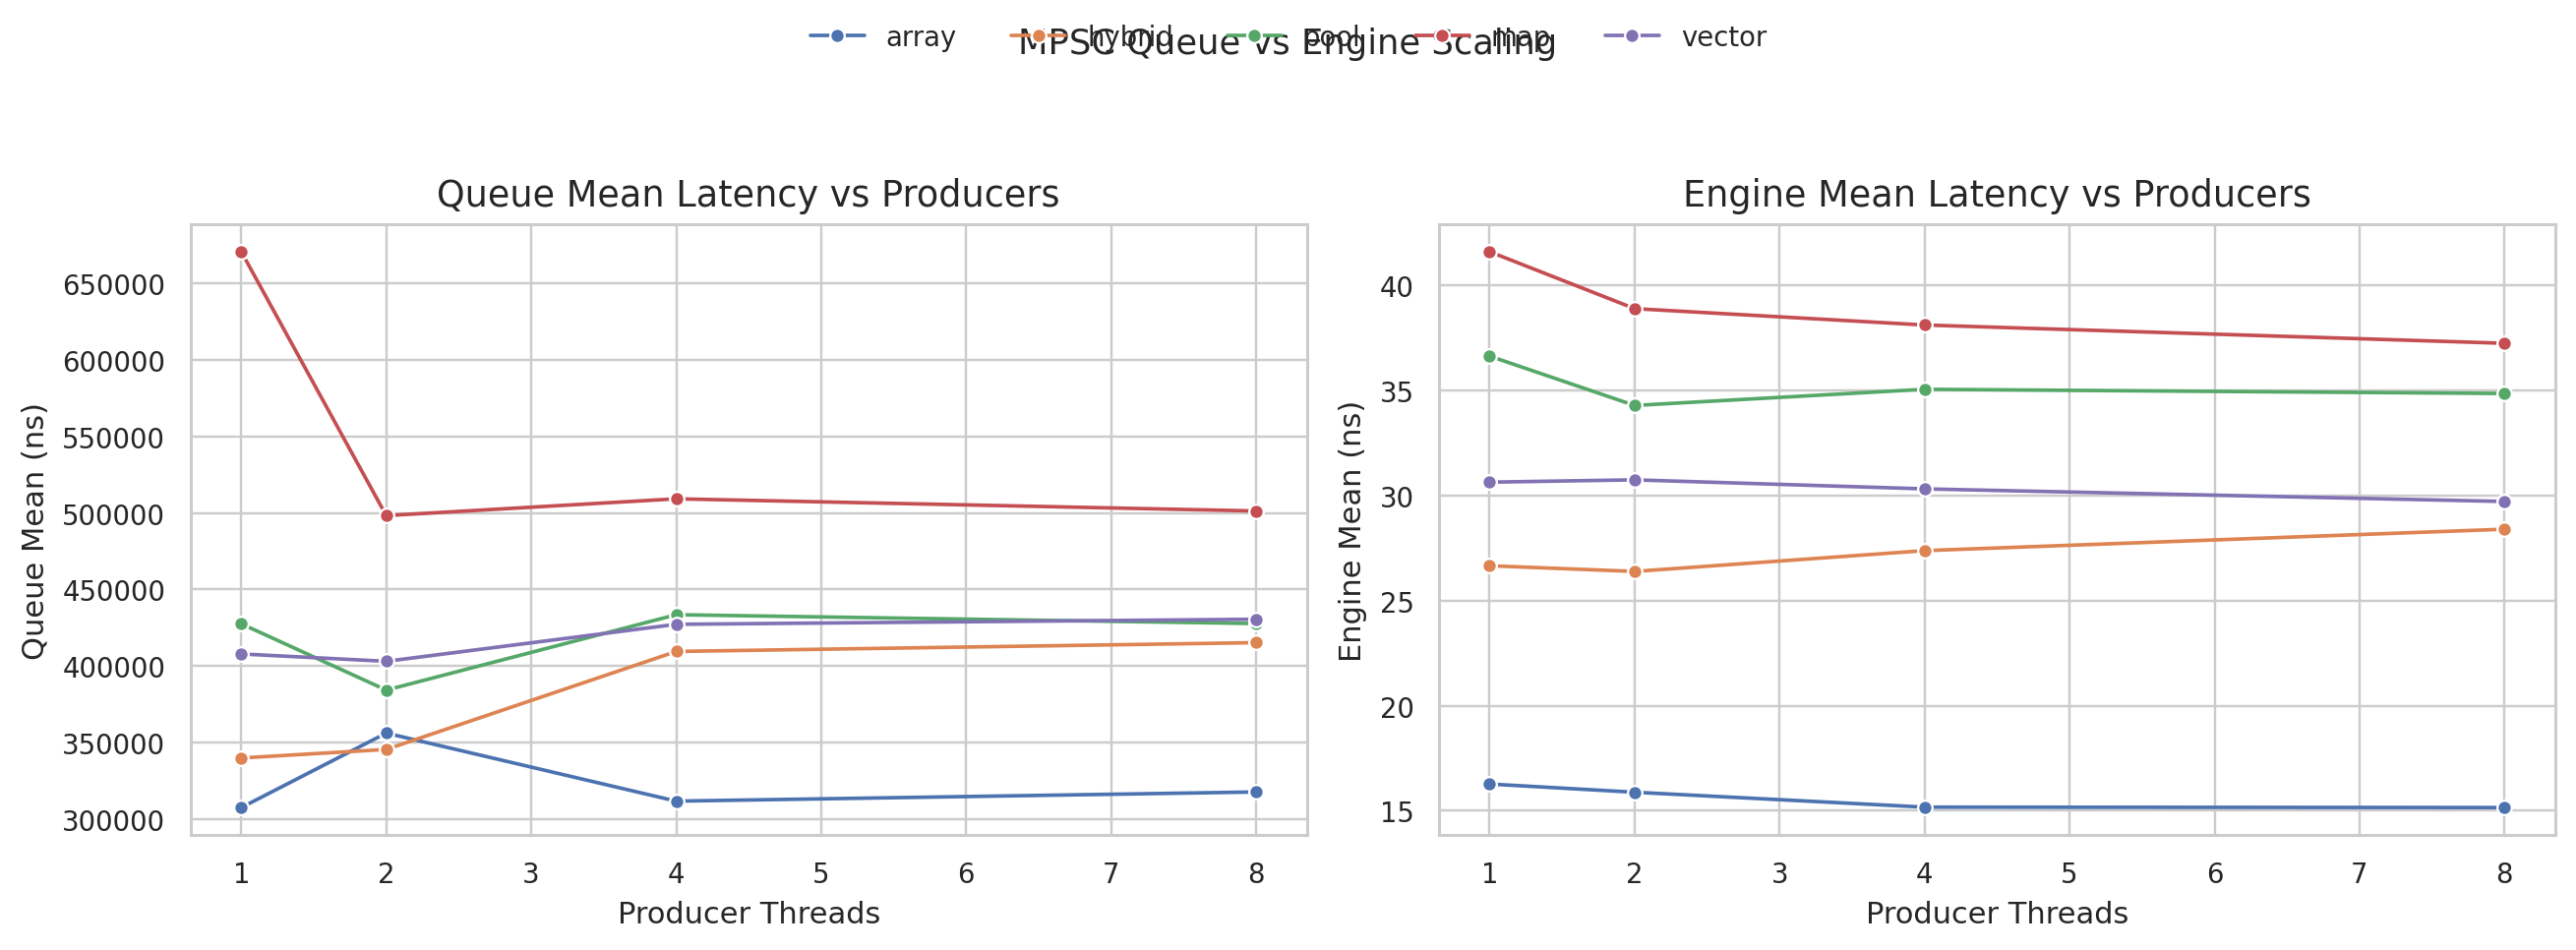
\includegraphics[width=0.8\textwidth]{../plots/mpsc/queue_vs_engine_scaling.png}
    \caption{Latency breakdown showing how queue wait times grow as more threads are added, while engine matching time stays the same.}
    \label{fig:mpsc_queue_latency}
\end{figure}

Figure~\ref{fig:mpsc_queue_latency} explains why this happens by breaking the 
latency down into queue time and engine time. 
The graph shows that the time an order spends waiting inside the queue is 
much higher than the time it takes the engine to actually process the order. 
For the array order book, the engine only needs about 15~ns to process an order, 
but that same order spends over 300,000~ns just sitting in the queue. 
This shows that when there is high traffic, the system is primarily limited by the 
speed of the single matching core. 
Because the producers are sending orders faster than the single matching engine 
can process them, the orders simply back up in the queue.
\section{Summary of Evaluation against Requirements}
\label{sec:nfr_summary}

The evidence gathered in these benchmarks addresses the project's requirements. 
Functional requirements for isolated metrics (\FR{2}) and end-to-end 
gateway tracking (\FR{3}) were met using the triple-timer design. 
For non-functional requirements, the identical test scenarios ensured 
fairness (\NFR{2}), while the code coverage confirmed semantic parity (\NFR{1}). 
These results successfully met the goals set for our system. 
They indicated that index-based layouts are faster internally (\NFR{3}), and they 
validated the system-level masking effect when operating over a network (\NFR{4}).

\section{Threats to Validity}
\label{sec:threats_to_validity}

While the benchmarks provide strong evidence, certain limitations must be noted 
to bound the validity of these results. 

\begin{itemize}
    \item \textbf{Virtualisation Overhead.}
        The use of WSL2 introduces a virtualisation tax due to the underlying 
        Hyper-V utility VM architecture~\citep{microsoft_wsl2_arch}. 
        While this environment adds inconsistent network jitter and I/O 
        overhead, the findings remain valid because 
        the penalty is applied equally across all implementations. 

    \item \textbf{Hardware Specificity.}
        The benchmarks were conducted on a Zen 4 AMD Ryzen 7600X 
        microarchitecture. 
        The specific cache sizes and branch predictor behavior of this processor 
        directly influence the recorded latency. 
        While the relative performance trends are likely to hold across modern 
        CPUs, the exact gaps may vary on server-grade Intel or AMD hardware. 

    \item \textbf{Synthetic Workloads.}
        The scenarios use randomized order flows that do not perfectly capture 
        the correlated bursts and strategic activity of a live market. 
        In a real-world exchange, clusters of activity at specific price levels 
        might stress the data structures in ways not captured by a uniform 
        random generator. 

    \item \textbf{Loopback Interface Limitations.}
        The Gateway mode uses the \texttt{127.0.0.1} interface, which 
        captures OS kernel overhead but lacks the physical delay of a 
        real network. In a production environment with discrete hardware, 
        latencies would likely be higher and more variable due to switch 
        buffering and NIC DMA processes.

    \item \textbf{CPU and Cache Contention.}
        In Gateway and MPSC modes, the producer (client) and consumer 
        (engine) share the same physical CPU socket. Despite thread-pinning, 
        there is inevitable contention for shared resources such as the 
        \textbf{L3 Cache} and the memory controller. This may slightly 
        inflate the recorded latencies compared to a separated production 
        environment where the engine is isolated on a dedicated server.

    \item \textbf{Statistical Sample Size.}
        A sample size of $n=5$ with 10,000 orders per scenario was used to 
        maintain a practical benchmark duration. 
        While this is sufficient for identifying major architectural trends, 
        a larger sample would be necessary for formal statistical significance 
        testing in a production setting. 
\end{itemize}

Despite these limitations, the evidence gathered in this chapter provides a 
consistent and clear evaluation of the trade-offs between order book 
implementations.

